\documentclass[12pt]{article}
%%% packages used %%%%%%%%%%%%%%%%%%%%%%%%%%%%%%%%%%%%%%
% avoid using extra packages
% we want the document as package free as possible
% as plain as possible
%\usepackage[utf8]{inputenc}
\usepackage[letterpaper]{geometry}

%% need these for math symbols
\usepackage{amsmath}
\usepackage{mathtools}

%% need this for listing authors
\usepackage{authblk}

%% need this for figures
\usepackage{graphicx}

%% comment hyperref package if needed
\usepackage{hyperref}

%% uncomment cite package to get auto complete
%% of citations
%%\usepackage{cite}
%%%%%%%%%%%%%%%%%%%%%%%%%%%%%%%%%%%%%%%%%%%%%%%%%%%
%%% comment two lines below to turn off line numbers %%%
\usepackage{lineno}
\linenumbers
%%%%%%%%%%%%%%%%%%%%%%%%%%%%%%%%%%%%%%%%%%%%%%%%%%%

%% to make hyperref clear, comment out
%% for final submission
\hypersetup{
    colorlinks=true,
    linkcolor=blue,
    citecolor = red,
    filecolor=magenta
    }
%%%%%%%%%%%%%%%%%%%%%%%%%%%%%%%%%%%%%%%%%%%%%%%%%%
%%% NO MACROS allowed!!!
%%% this gives the keywords part --> may need to remove
\providecommand{\keywords}[1]{\textbf{\textit{Keywords:}} #1}
%% these are the commands for the calcium concentration symbols --> not allowed, no macros!!
%\newcommand{\Ca}{$\textrm{Ca}^{2+}$}
%\newcommand{\CaCon}{$[\textrm{Ca}^{2+}]\ $}
%\newcommand{\Na}{$\textrm{Na}^+$}

%% this sets row height in tables
%%\renewcommand{\arraystretch}{1.25}

%% added a footnote on first page
%%\renewcommand{\thefootnote}{\fnsymbol{footnote}}

%% this is for setting line number sizes comment this out later!
\renewcommand\linenumberfont{\normalfont\bfseries\scriptsize}

\makeatletter 
\renewcommand\@biblabel[1]{\textbf{#1.}} 
\makeatother
%%%%%%%%%%%%%%%%%%%%%%%%%%%%%%%%%%%%%%%%%%%%%%%%%%
%% the title and author fonts were 
%% unnecessarily big compared to the rest of 
%% the document
\font\titlefont=cmr12 at 16pt
\font\authorfont=cmr12 at 12pt
%%% beginning of article %%%%%%%%%%%%%%%%%%%%%%%%%%%%%%%
\title{\vspace{-3em}\titlefont Calcium modeling of spine apparatus-containing human dendritic spines demonstrates ``all-or-nothing" communication switch between the spine head and dendrite}
\author[1,$\ast$]{\authorfont James Rosado}
\author[2,$\ast$]{\authorfont Viet Duc Bui}
\author[3,4,5,6]{\authorfont Carola A. Haas}
\author[3,6]{\authorfont J\"urgen Beck}
\author[1,$\$$,\S]{\authorfont Gillian Queisser}
\author[2,4,5,6,$\$$,\S]{\authorfont Andreas Vlachos}
\affil[1]{\authorfont Department of Mathematics, Temple University, Philadelphia, USA}
\affil[2]{\authorfont Department of Neuroanatomy, Institute of Anatomy and Cell Biology, Faculty of Medicine, University of Freiburg, Freiburg, Germany}
\affil[3]{\authorfont Department of Neurosurgery, Medical Center-University of Freiburg, Faculty of Medicine, University of Freiburg, Freiburg, Germany}
\affil[4]{\authorfont Bernstein Center Freiburg, University of Freiburg, Freiburg, Germany}
\affil[5]{\authorfont Center Brain Links Brain Tools, University of Freiburg, Freiburg, Germany}
\affil[6]{\authorfont Center for Basics in NeuroModulation (NeuroModulBasics), Faculty of Medicine, University of Freiburg, Freiburg, Germany}
\affil[$\ast$]{\authorfont These authors contributed equally to this work}
\affil[$\$$]{\authorfont Joint senior authors}
\affil[$\S$]{\authorfont Correspondence to gillian.queisser@temple.edu and andreas.vlachos@anat.uni-freiburg.de}
\date{}

\begin{document}

\maketitle

%\footnotetext[1]{These authors contributed equally to this work}
%\footnotetext[2]{Joint senior authors}
%\footnotetext[4]{Correspondence to gillian.queisser@temple.edu and andreas.vlachos@anat.uni-freiburg.de}
\vspace{-3em}
\clearpage
\begin{abstract}
    Dendritic spines are highly dynamic neuronal compartments that control the synaptic  transmission between neurons. Spines form ultrastructural units, coupling synaptic contact sites to the dendritic shaft and often harbor a spine apparatus organelle, composed of smooth endoplasmic reticulum, which is responsible for calcium sequestration and release into the spine head and neck. The spine apparatus has been linked recently to synaptic plasticity in adult human cortical neurons. While the morphological heterogeneity of spines and their intracellular organization has been extensively demonstrated in animal models, the influence of spine apparatus organelles on critical signaling pathways, such as calcium-mediated dynamics, is less well known in human dendritic spines. In this study we used serial transmission electron microscopy to carry out detailed anatomical reconstructions of nine human cortical spines in order to quantify and analyze the architectural plan of the spines and to incorporate the reconstructions into detailed modeling and simulation of the calcium dynamics between spine and dendrite. The anatomical study of reconstructed human dendritic spines revealed that the size of the postsynaptic density correlates with spine head volume and that the spine apparatus volume increases alongside the spine volume. Using a newly developed simulation pipeline, we have linked these findings to spine-to-dendrite calcium communication. While the absence of a spine apparatus, or the presence of a purely passive spine apparatus did not enable any of the reconstructed spines to relay a calcium signal to the dendritic shaft, the calcium-induced calcium release from this intracellular organelle allows for finely tuned ``all-or-nothing" spine-to-dendrite calcium coupling; controlled by spine morphology, neck plasticity, and ryanodine receptors. Our results suggest a  strategic position of spine apparatus organelles in the neck of human dendritic spines and their potential relevance in maintaining and regulating spine-to-dendrite calcium communication.
\end{abstract}
\keywords{calcium, dendritic spines, endoplasmic reticulum, intracellular calcium stores, Ryanodine receptors, human cortex}
\clearpage
\section*{Introduction}
Calcium-based second-messenger signaling pathways mediate fundamental biological processes in the human body \cite{Berridge2000}. In the brain, synaptically evoked intracellular $\textrm{Ca}^{2+}$  surges regulate the ability of neurons to adjust their synaptic contacts in an activity-dependent manner \cite{Holthoff2006,Higley2008}. This fundamental biological mechanism (i.e., synaptic plasticity), plays a crucial role in complex brain functions, such as internal representation and memory formation \cite{Sala2014,Padamsey2019}. Over the past few decades, cellular and molecular mechanisms of $\textrm{Ca}^{2+}$ dependent synaptic plasticity have been extensively studied in dendritic spines across various animal models \cite{Higley2012, Maggio2014}.  

Dendritic spines are highly dynamic neuronal compartments on which cortical excitatory synapses are typically formed \cite{Yuste1995,Amaral2009}. Most spines have a bulbous head and a thin neck that connects the spine head to the shaft of the dendrite. Additionally, they often harbor a dynamic extension of the smooth endoplasmic reticulum (sER) in the dendrite, which can rapidly enter and leave the spine compartment and is capable of changing its position inside the neck and head of spines \cite{PerezAlvarez2020}. Indeed, they play a critical role in sER intracellular $\textrm{Ca}^{2+}$ storage and in synaptic plasticity \cite{Verkhratsky2005,Vlachos2009,Holbro2009,Korkotian2014}.  The variable nature of spine morphology and intracellular $\textrm{Ca}^{2+}$ stores has been studied with respect to electrical and biochemical signaling \cite{Tonnesen2016, Nishiyama2015, Cartailler2018}. More recent research has studied the influence of synaptic spine architecture on calcium signaling by parametrically designing the leading features of spines (i.e., spine neck width/length, spine head volume, and the size of the sER) and performing computational studies on a wide variety of such synthetically designed geometries \cite{Bell2019, Basnayake2019, Breit2018}.	

Guided by the existing literature and our own recent work \cite{Breit2018, BreitQ2018, Lenz2021}, we carried out detailed anatomical reconstructions of human cortical spines based on serial transmission electron microscopy and performed a correlation analysis on a set of geometric features, including the size and position of the postsynaptic density (PSD), spine head volumes, and cross-sectional areas of the spine neck. We then attempted to answer how the distinct three-dimensional ultrastructural organization of human dendritic spines influences intracellular $\textrm{Ca}^{2+}$ dynamics in the spine head and neck, and how these signals propagate into the attached dendritic shaft (i.e., spine-to-dendrite $\textrm{Ca}^{2+}$ communication). Specifically, we wanted to learn more about the role of the spine apparatus organelle (SA) \cite{GRAY1959, Spacek1985, Spacek1997}, an enigmatic cellular organelle composed of stacked sER, found in the majority of cortical dendritic spines in humans \cite{Lenz2021}.


\section*{Results}
\subsection*{Spine $\textrm{Ca}^{2+}$ modeling in reconstructed human dendritic spines containing a spine apparatus organelle}
To capture the effect of the SA on $\textrm{Ca}^{2+}$ dynamics in dendritic spines, the three-dimensional architecture of dendritic spines, including intracellular membrane structures, must be carefully considered. Expanding on the results obtained from synthetically generated dendritic spines \cite{Breit2018}, we reconstructed detailed morphologies of nine dendritic spines%shown in Figure \ref{fig:fig2}A
, their SA, and postsynaptic densities from cortical surgical access material using serial transmission electron microscopy (TEM). From the serial TEM image stacks, we then generated realistic three-dimensional geometric models, see Figures \ref{fig:fig1}A and \ref{fig:fig1}B.

Immunogold staining for the actin-binding protein synaptopodin, which is an essential component for the formation of the SA in the rodent brain \cite{Deller2003}, confirmed that the actin-modulating protein synaptopodin is a marker for human SA (Figure \ref{fig:fig1}C; c.f.,\cite{Lenz2021}). We then attached the reconstructed SAs to a single standardized dendritic ER tubule in a dendritic compartment of identical dimensions for all spines (Figure \ref{fig:fig1}D). We used the resulting surface triangulation of the plasma membrane, the SA, the PSD, and dendritic ER to construct a volumetric tetrahedral mesh \cite{Si2015} for numerical simulations.

Next, we adapted and integrated existing single-channel models of $\textrm{Ca}^{2+}$ exchangers in the plasma membrane - i.e., plasma membrane $\textrm{Ca}^{2+}$-ATPase (PMCA) and $\textrm{Na}^{+}$/$\textrm{Ca}^{2+}$ exchangers (NCX), as well as Ryanodine receptors (RyR) on the SA membrane (see schematics in Figure \ref{fig:fig1}E) - into a diffusion-reaction model for cytosolic and endoplasmic $\textrm{Ca}^{2+}$ dynamics \cite{Breit2018}. Numerical simulations were carried out on computational domains defined by the reconstructed human dendritic spine morphologies, using established numerical methods (details provided in Methods).

\subsection*{Spine apparatus-containing human dendritic spines showed larger spine head volumes and postsynaptic densities}
We recently showed that $\sim$70\% of all dendritic spines on human layer II/III pyramidal neurons contain a synaptopodin cluster (i.e., SA) \cite{Lenz2021}. By carefully examining EM cross-sections, we obtained evidence that large human dendritic spines contain SA organelles \cite{Lenz2021}, which is consistent with earlier work conducted on synaptopodin clusters, SA, and spine head sizes of neurons in rodent brains \cite{OkuboSuzuki2008, Vlachos2009, Vlachos2013,Yap2020}. However, no three-dimensional analyses of SA-containing human dendritic spines have been performed thus far. 

To test whether there are correlations between the reconstructed spine components, we carefully examined critical morphological parameters of the reconstructed SA-containing dendritic spines (Figure \ref{fig:fig2}). Consistent with previous studies in animal models \cite{Harris1989,Arellano2007}, a positive correlation between PSD sizes and spine volumes was observed in the spines reconstructed from human cortical tissue (Figure \ref{fig:fig2}B). This relation was readily detected when spines were sorted by spine head volume. Moreover, we observed a positive correlation between PSD sizes and cross-sectional areas of spine necks (Figure \ref{fig:fig2}C). This finding raises the possibility that larger spines with a wider neck may allow for a more effective $\textrm{Ca}^{2+}$ spine-to-dendrite communication. 

Following the major scope of this study (i.e., the modeling of spine-to-dendrite $\textrm{Ca}^{2+}$ communication), we determined distances between PSDs and the dendritic compartment. Figure 2D shows no significant correlation between spine volumes and PSD-to-dendrite distances, which were defined as the Euclidian distance between the point of the PSD closest to the base of the spine. These results indicated that SA-containing spines of the human cortex may differ in their volume and spine neck diameters, while PSD-to-dendrite distances are comparable; at least, for the nine reconstructed spines used in this study. 

Finally, we examined the morphological properties of the SAs contained in the reconstructed spines (Figure \ref{fig:fig2}E). We observed a positive correlation between spine volume and SA volume, which was also observed when spine neck cross-sections were considered. These results provided ultrastructural morphological insight into the three-dimensional organization of SA-containing dendritic spines in the human cortex. They support the previously proposed spine-within-a-spine ER morphology, which plays the leading role governing spine volume and sER volume ratio in $\textrm{Ca}^{2+}$ signaling \cite{Berridge2000,Bell2019}. 

\subsection*{Passive spine apparatus organelles have no major impact on spine-to-dendrite $\textrm{Ca}^{2+}$ signaling}
To assess the role of the SA in spine-to-dendrite $\textrm{Ca}^{2+}$ communication, we first investigated $\textrm{Ca}^{2+}$ signal propagation in spines for which the reconstructed SA was excluded. In all simulations the same $\textrm{Ca}^{2+}$ ion flux $(j_c^{rls})$ was used for the PSD at the spine head, \cite{Keller2008,Higley2012}, see Table \ref{table4} for the flux value. Changes in $[\textrm{Ca}^{2+}]$ were measured in three regions of interest: the spine head, spine neck, and the dendrite \cite{Breit2018}. For all of our numerical experiments we simulated an AMPA model at the PSD with a 10 ms release of $\textrm{Ca}^{2+}$ by a linearly decreasing $\textrm{Ca}^{2+}$ pulse, described further in the \textit{methods} section. The number of ions released at the PSD for each spine %is given in Table \ref{table1} and 
is computed by
\[
\#\ \textrm{of ions} = \left\lfloor N_A\cdot \int_0^{\tau_{rls}}j_c^{rls}\cdot\left(1-\frac{t}{\tau_{rls}}\right)\cdot A_{PSD}\ dt\right\rfloor,
\]
where $A_{PSD}$ is the area of the PSD, and $N_A= 6.02214076\times 10^{23}\  \textrm{mol}^{-1}$ is Avogadro's constant.

As shown in Figure \ref{fig:fig3}A, only a small fraction of released $\textrm{Ca}^{2+}$ ions reached the dendritic compartment. To quantify the dendritic response to $\textrm{Ca}^{2+}$ release at the PSD, the $[\textrm{Ca}^{2+}]$ amplitude was measured in the spine head, neck and dendrite. The values and ratios between head and dendrite amplitude for all spines are listed in Table \ref{table2}. In all cases less than 3\%  of the initial $[\textrm{Ca}^{2+}]$ amplitude in the head was detectable in the dendrite. When the SA was added as a passive cellular compartment (i.e., when it was present as a geometric obstacle, but without any $\textrm{Ca}^{2+}$ exchange mechanisms that would allow $\textrm{Ca}^{2+}$ exchange across the SA membrane), similar and near-zero dendritic $[\textrm{Ca}^{2+}]$ profiles were observed in the respective spines (Figure \ref{fig:fig3}B). Minor differences in the profiles (compared to the no-SA case) can be observed in the head and neck; however, these all lie in the single-digit $\mu\textrm{mol}/l$ range. 

The differences in peak $[\textrm{Ca}^{2+}]$ amplitude between passive-SA and no-SA are presented in Figure \ref{fig:fig3}C–E. These differences decreased with increasing spine volume (Figure \ref{fig:fig3}C) and are positively correlated to the SA/Spine volume ratio (Figure \ref{fig:fig3}D). Two clear outliers in this trend are spines 1 and 4. To test whether the SA is able to block $\textrm{Ca}^{2+}$ passage at the intersection between head and neck \cite{Biess2011}, and thus produce larger differences in the $[\textrm{Ca}^{2+}]$ amplitude, the data was plotted against the SA/spine surface area ratio at this intersection (Figure \ref{fig:fig3}E). The outlier, spine 4, could clearly be explained by this metric. Thus, accumulation of SA in the intersectional region between head and neck may obstruct $\textrm{Ca}^{2+}$ diffusion. Numerical simulations were also carried out for PSD adjusted $\textrm{Ca}^{2+}$ influx (see Figure \ref{fig:fig7})- i.e. $\textrm{Ca}^{2+}$  influx was scaled by PSD surface area, using spine 8 as the reference spine. It should be noted that PSD-adjusted $\textrm{Ca}^{2+}$ influx may compensate for the $\textrm{Ca}^{2+}$ accumulation in the head region. In Figure \ref{fig:fig7}, for example, the change in $[\textrm{Ca}^{2+}]$ remains relatively uniform when correlated against spine volume, with the exception of spine 4 for which we observe the above -described “corking effect”. Taken together, from these results (fixed $\textrm{Ca}^{2+}$ and PSD-adjusted), we can conclude that spine-to-dendrite $\textrm{Ca}^{2+}$ signaling in the dendrite is negligible for both the no-SA and the passive-SA setting. These observations strengthen the case for active $\textrm{Ca}^{2+}$ exchange across the spine ER membrane in order to enable spine-to-dendrite $\textrm{Ca}^{2+}$ communication in SA-containing dendritic spines.

\subsection*{Ryanodine receptors of spine apparatus control spine-to-dendrite $\textrm{Ca}^{2+}$ signaling}
Previous work revealed that RyR-dependent $\textrm{Ca}^{2+}$-induced $\textrm{Ca}^{2+}$ release from synapto-podin-associated $\textrm{Ca}^{2+}$ stores modulates spine $\textrm{Ca}^{2+}$ dynamics and synaptic plasticity \cite{Vlachos2009,Korkotian2014,Maggio2014}. To assess the role of active SAs in human dendritic spines, by including RyRs on the membrane of the SA and dendritic ER, we determined the critical RyR density for spine-to-dendrite $\textrm{Ca}^{2+}$ communication for each spine (Table \ref{table1}). To quantify spine-to-dendrite $\textrm{Ca}^{2+}$ coupling, we defined the peak $[\textrm{Ca}^{2+}]$ to be a concentration value greater than $1\  \mu \textrm{mol}/l$ in the dendritic measuring zone for 1 ms. Converting this concentration minimum (during 1 ms) leads to $1\times 10^{-18}\ \textrm{mol}/(s\cdot\mu m^3)$, and then multiplying by the width of the dendrite ($\sim 1\ \mu m$) obtains an approximate flux through the neck-dendritic interface of $1\times 10^{-18}\ \textrm{mol}/(s\cdot \mu m^2)$. Therefore, we defined a spine-to-dendrite coupling as successful if more than $11\%$ of the initial $\textrm{Ca}^{2+}$ influx at the PSD was measured in the dendrite (using $8.6\times 10^{-18}\ \textrm{mol}/(s\cdot \mu m^2)$ for reference). We increased the RyR density in 0.01 $\mu m^{-2}$ increments in the range of 0–5 RyRs $\mu m^{-2}$ and found critical RyR values for all reconstructed morphologies, ranging between 1.37 and 3.5 $\mu m^{-2}$ (Table \ref{table1}). Figure \ref{fig:fig4}A shows all spines eliciting dendritic $\textrm{Ca}^{2+}$ coupling when the critical RyR density is surpassed. A small number of RyRs on SAs (i.e., 1–6 receptors) was sufficient to enable spine-to-dendrite $\textrm{Ca}^{2+}$ communication, see Table \ref{table1}. However, the peak $[\textrm{Ca}^{2+}]$ drops below 1 $\mu\textrm{mol}/l$ when the RyR density is subcritical (Figure \ref{fig:fig4}B). Thus, RyR density plays a critical role in spine-to-dendrite $\textrm{Ca}^{2+}$ coupling.

We next tested whether changes in $\textrm{Ca}^{2+}$ entry at the PSD affect the critical RyR density by successively increasing the $\textrm{Ca}^{2+}$ flux density at the PSD entry site. However, coupling occurs at the same RyR density, independent of the initial $\textrm{Ca}^{2+}$ influx within the range $8.6\times 10^{-18}-22.0\times 10^{-18}\ \textrm{mol}/(s\cdot \mu m^2)$ tested here, see Figures \ref{fig:fig4}C-D for spine 8 as an example. This invariance can be attributed to intracellular $\textrm{Ca}^{2+}$ buffering, as modifications in the buffering capacity produced a shift in the critical RyR density. This was observed when we ran our simulations with half the buffering capacity (Figure \ref{fig:fig4}E), which caused a small decrease in the critical RyR density. It is also worth clarifying that the transition between coupling and decoupling spine-to-dendrite $\textrm{Ca}^{2+}$ signals is highly nonlinear (see jumps in Figures \ref{fig:fig4}C-E). Changes in critical RyR density appear to control the ``all-or-nothing" $\textrm{Ca}^{2+}$ dynamics in the parent dendrite. 

Comparing the peak calcium concentrations of passive and active SA in the head and dendrites (see Table \ref{table2}) showed that the relative differences between passive and active ER dynamics are the result of $\textrm{Ca}^{2+}$-induced $\textrm{Ca}^{2+}$ release through RyRs, which releases additional $\textrm{Ca}^{2+}$ into the cytosol \cite{Johenning2015}. While the critical RyR density was not dependent on $\textrm{Ca}^{2+}$ influx at the PSD, we further analyzed whether the structural organization of dendritic spines could play a role. For completeness, we provided $\textrm{Ca}^{2+}$ profiles (see Figure \ref{fig:fig6}) for PSD-adjusted $\textrm{Ca}^{2+}$ influx at both critical RyR and subcritical RyR densities.
%, and with SERCA pumps.


\subsection*{Spine morphology and neck plasticity affect spine-to-dendrite \\ $\textrm{Ca}^{2+}$ signaling}
Critical for endoplasmic $\textrm{Ca}^{2+}$ release through RyRs is having sufficient $[\textrm{Ca}^{2+}]$ at the endoplasmic membrane \cite{Emptage1999,Korkotian1999,Korkotian2014}. Thus, an intracellular organization of the SA that would support sufficient accumulation of $\textrm{Ca}^{2+}$ at the spine neck (the most confined part of the spine morphology) should reduce the critical RyR density. To test this hypothesis, the critical RyR density was plotted against the ratio of SA in the spine neck to the spine neck cross-sectional area (Figure \ref{fig:fig5}A). We found that the area ratio correlated negatively with the RyR density, demonstrating that a smaller RyR density is sufficient to induce spine-to-dendrite coupling when the SA occupies larger portions of the spine neck.
		
Interestingly, we observed a positive correlation between the spine and SA cross-sectional area of the spine neck (Figure \ref{fig:fig5}B), suggesting that the SA adjusts to dendritic spine growth and reorganizes in such a way to support spine-to-dendrite $\textrm{Ca}^{2+}$ communication. Previous work has demonstrated that changes in spine neck diameters accompany the induction of excitatory synaptic plasticity, reflected by an increase in spine head size \cite{Araya2014,Tonnesen2014,Steffens2021}. Specifically, spine necks are shortened and widened after long-term potentiation of excitatory neurotransmission \cite{Tonnesen2014}. 
		
We therefore systematically tested whether changes in spine neck diameter can affect spine-to-dendrite $\textrm{Ca}^{2+}$ communication. To address the role of spine neck plasticity in spine-to-dendrite $\textrm{Ca}^{2+}$ communication, we ran simulations by using the reconstruction of spine 6, and manually widening the spine neck by 10\%, 20\%, and 40\%, while keeping the RyR density and the SA morphology constant (Figure \ref{fig:fig5}, modified spines 6-A, 6-B, 6-C, respectively). While the $\textrm{Ca}^{2+}$ dynamics in the spine head remained unchanged (Figure \ref{fig:fig5}C), we observed that increasing the spine neck width caused a decrease in peak $\textrm{Ca}^{2+}$ near the SA membrane, thereby producing insufficient $\textrm{Ca}^{2+}$ release from the SA store to maintain spine-to-dendrite coupling (Figure \ref{fig:fig5}D). 
		
We then tested whether an increase in RyR density could balance morphological plasticity in order to maintain coupling even under spine growth and reorganization. For each of the modified spines 6-A, 6-B, and 6-C, we incrementally increased the RyR density and observed that a critical RyR density can be determined for all spines. Naturally, this critical value increases with increasing neck width, see Figure \ref{fig:fig5}E (critical RyR densities for spines 6-A, 6-B, 6-C can be found in Table \ref{table1}). We have not tested whether increasing the size of the SA restores spine-to-dendrite communication. The current results appear to suggest that for a SA with subcritical RyR density, increasing the SA size will restore spine-to-dendrite communication.
		
This means, that not only could coupling be restored but, as Figure \ref{fig:fig5}F shows, the dendritic $\textrm{Ca}^{2+}$ profiles for all adjusted spines are nearly identical, indicating that $\textrm{Ca}^{2+}$ is sensitive to changes in spine neck and SA morphology in human dendritic spines, and  that $\textrm{Ca}^{2+}$ dynamics are affected by spine neck and SA geometry \cite{Svoboda1996,Biess2007,Noguchi2005}.

In conclusion, we observed an ``all-or-nothing'' $\textrm{Ca}^{2+}$ communication switch between spine head and dendrite that is controlled by an interplay between RyR density and morphological changes of dendritic spines and SAs. 


\section*{Discussion}
In this study, we explored spine $\textrm{Ca}^{2+}$ dynamics in human cortical spines using simulations consisting of (i) $\textrm{Ca}^{2+}$ diffusion and reaction with mobile calcium buffer (calbindin, CalB) in the cytosol; (ii) $\textrm{Ca}^{2+}$ diffusion inside the SA and sER of the dendrite; and (iii) $\textrm{Ca}^{2+}$ exchange across the plasma (PMCA, NCX) and endoplasmic (RyR) membranes (Figure \ref{fig:fig1}E). We showed that a critical RyR density, dependent on the overall spine and SA architecture, allows active $\textrm{Ca}^{2+}$-induced $\textrm{Ca}^{2+}$ release to maintain spine-to-dendrite $\textrm{Ca}^{2+}$ communication. Increasing the neck diameter or decreasing the SA cross-sectional area in the neck region of individual spines disrupts this communication pathway. Increasing the RyR density (or SA sizes) can reverse this effect (Figure \ref{fig:fig8}). These findings suggest a critical role for SA- and spine neck plasticity in controlling $\textrm{Ca}^{2+}$ communication between the spine head and dendrite.

The ability to visualize individual dendritic spines in living brain tissue over extended periods was developed three decades ago \cite{Guthrie1991, MullerConnor1991}. Consequently, the amount of information about the morphology and physiology of dendritic spines and the molecular mechanisms acting on spines has increased tremendously \cite{Svoboda1996,Sabatini2002,Holtmaat2005,Sala2014,Segal2017}. However, major issues regarding structure-function interrelations and the role of dendritic spines in network function and complex behavior remain unresolved \cite{Segal2017}. This is particularly true for structure-function interrelations in the human cortex, which are beginning to emerge \cite{Lenz2021}. In adult human neurons, it is currently not possible to carry out the required experiments to study spine $\textrm{Ca}^{2+}$ dynamics as they require genetic tools for simultaneous visualization of dendritic spines, SAs and changes in intracellular $\textrm{Ca}^{2+}$ levels. Also, it is impossible to systematically assess the relevance of individual spine and SA/ER parameters, as they are not easy to manipulate in biologically complex systems.  In this respect, computer simulations based on serial EM reconstructions provide suitable tools to explore spine $\textrm{Ca}^{2+}$ dynamics in human dendritic spines.
	
Our morphological analyses of the nine reconstructed spines used in this study confirm and expand on our recent findings on dendritic spine plasticity of layer II/III pyramidal neurons in the adult human cortex \cite{Lenz2021}. In this earlier study, we showed that (i) approximately 70\% of dendritic spines contain synaptopodin clusters; (ii) synaptopodin clusters and spine apparatus organelles are found in dendritic spines with large cross-sectional areas; and (iii) a plasticity-inducing stimulus promotes remodeling of synaptopodin clusters, spine apparatus organelles, and dendritic spines in human cortical neurons. These changes correlated well with changes in spontaneous excitatory postsynaptic currents recorded from individual layer II/III pyramidal neurons \cite{Lenz2021}. Consistent with these earlier findings, we confirmed in this study that synaptopodin is a marker for the human SA, and we also demonstrated a positive correlation between SA volumes, PSD sizes, and spine volumes. Although we concede that this analysis is currently based only on nine reconstructed spines, disclosing such interrelation with comparably small numbers indicates that these morphological measures may be tightly regulated in the human cortex. 
	
Our simulations using a purely passive SA, strengthen the case for active $\textrm{Ca}^{2+}$ exchange across the spine ER membrane to enable spine-to-dendrite $\textrm{Ca}^{2+}$ communication in SA-containing dendritic spines. Specifically, choosing a critical RyR density enabled spine-to-dendrite $\textrm{Ca}^{2+}$ communication. This RyR density depended on the overall spine and SA architecture, while being independent of the strength of the initial $\textrm{Ca}^{2+}$ influx through the PSD. By increasing spine neck sizes for individual spines this communication pathway was disrupted. Increasing the RyR density, or adjusting SA to spine-neck ratios, however, reversed this effect.  While the actual RyR densities and changes in the number of RyRs on ER membranes remain unknown, changes in spine neck sizes and spine apparatuses (both sizes and position within a spine) are well described \cite{Vlachos2009,Vlachos2013,Tonnesen2014,PerezAlvarez2020,Yap2020}. Hence, the physiology and morphology of dendritic spines appear tightly integrated and can control $\textrm{Ca}^{2+}$ communication between the spine head and dendrite. In this context, the SA may serve $\textrm{Ca}^{2+}$ homeostasis in maintaining spine-to-dendrite $\textrm{Ca}^{2+}$ communication during dendritic spine growth as seen after plasticity induction. Conversely, it is interesting to theorize that changes in SA sizes or position within the spine may allow for rapid input-specific control of spine $\textrm{Ca}^{2+}$ signals. Whether such mechanisms serve input-specific synaptic plasticity, $\textrm{Ca}^{2+}$ dependent local dendritic protein synthesis \cite{Swanger2013}, synaptic tagging \cite{Martin2002,Park2019}, or other as yet unknown mechanisms warrants further investigation. It may be important to mention in this context, however, that in our recent study we showed that blocking protein synthesis with anisomycin halted plasticity induction, dendritic spine, and SA growth in adult human cortical neurons \cite{Lenz2021}, suggesting a role of local protein synthesis in SA-dependent synaptic plasticity. 
	
Interestingly, the transition between coupling and decoupling of spine-to-dendrite $\textrm{Ca}^{2+}$ signals was highly nonlinear. This “all-or-nothing” property observed in our simulations is reminiscent of the physiological function of another cellular compartment in which synaptopodin-associated stacked ER is present: the axon initial segment and the cisternal organelle \cite{Palay1968,Somogyu1976,Benedeczky1994,BasOrth2005,Rasband2010,SanchezPonce2011}. Like SAs, cisternal organelles consist of flat, membrane-delineated cisternae alternating with electron-dense material. Similarly, synaptopodin-deficient mice do not form SAs and cisternal organelles \cite{BasOrth2005}. Indeed, from an anatomical point of view the analogy between spine heads and spine necks, and the soma and axon initial segment is striking. However, while the role of SA in spine calcium dynamics and synaptic plasticity seems well-established, the biological significance of cisternal organelles and their role in AIS-plasticity \cite{Grubb2010,PanVazquez2020, Jamann2021} remains less understood. It is probable that increased use of new electron microscopy techniques on human cortical tissue, such as focused ion beam, block-face serial electron microscopy, and array tomography, together with computer-based automatic 3D reconstructions will allow us to advance toward a better understanding of ultrastructure-function relations of synaptopodin associated stacked smooth ER in distinct neuronal compartments, and to test the extent to which data obtained from animal models translates to the adult human brain. 

\section*{Methods}
\subsection*{Ethics statement} Human brain tissue was obtained from a local biobank operated in the Department for Neurosurgery at the Faculty of Medicine, University of Freiburg Germany (AZ 472/15\_160880). All procedures were carried out after positive evaluation by the local ethics committee (AZ 593/19).
\subsection*{Electron microscopy} Tissue was fixed in 4\% paraformaldehyde (w/v) and 2\% glutaraldehyde (w/v; phosphate buffered saline) overnight. After fixation tissue was cut into 100 $\mu$m thin slices, thoroughly washed in phosphate buffer (0.1M) and incubated with 1\% osmium tetroxide for 60 minutes. After washing in graded ethanol (up to 50\% /v/v)) for 10 minutes each, slices were incubated with uranyl acetate (1\% (w/v) in 70\% (v/v) ethanol) overnight. Slices were then dehydrated in graded ethanol (80\%. 90\%, 96\% for 10 minutes each, and 2x 100\% for 10 minutes). After two washing steps in propylene oxide for 5 minutes each, the slices were incubated with durcupan/propylenoxid (1:1 for 1 hour) following durcupan only overnight at room temperature. Ultrathin sections of 20 - 40 nm were prepared at a Leica UC6 Ultracut. Sections were mounted into copper grids (Plano) and contrasted using Pb-citrate for 3 minutes. Transmission electron microscopy was performed at a Zeiss Leo 906 equipped at 6000x magnification. In total, cortical access tissue from 7 individuals who underwent clinically indicated neurosurgical procedures, e.g., for tumors or epilepsy, were processed and 1 to 6 acquisitions were obtained from each patient. Each acquisition included at least one labeled dendritic segment and synaptic contact. Up to 40 images of the same dendritic spines on consecutive sections were acquired and saved as TIF-files.
\subsection*{3D-reconstrunction of dendritic spines and generation \\ of spine models} Image series were adjusted in brightness and contrast using the Fiji software package \cite{Schindelin2012}. Stack alignment and segmentation were performed with the integrated TrakEM2 plugin \cite{Cardona2012}. For this purpose, an automatic alignment (rigid registration) was utilized followed by manual correction. Independent traces were drawn manually for each spine attached to a dendritic segment, spine apparatus organelles and postsynaptic densities. Dendritic spines possessing spine apparatus organelles that were complete within the series were reconstructed. A total of 9 series met these criteria and were used in analysis. The image segmentation binary files were transformed into a preliminary surface mesh using a Java 3D library \cite{Schmid2010} and saved in an `OBJ' format. However, meshes generated in this manner contained various mesh artifacts, such as jagged boundaries, non-manifold features and surface intersections. Using the meshing software ProMesh \cite{Reiter2012} for post-processing, including Laplacian smoothing, optimized surface meshes, compatible with physical simulations, were produced. Mesh defects, such as disconnects in the spine apparatus organelle due to thickness in ultrathin section or errors in the segmentation, were manually identified and matched to the cellular structures. Spine structures were manually subdivided into head and neck region after visual inspection of the 3D model from different angles. All reconstructed spines, including their spine apparatus organelles, were cut from their parent dendritic shaft through the base of the spine neck. Subsequently, they were attached to an dendritic segment containing the endoplasmatic reticulum. Using this method, we inserted spine apparatuses into reconstructed human spine models and generated hybrids of anatomical morphologies. Using ProMesh, we measured volumes from the three-dimensional reconstructions. While spine neck length was measured from the center of the spine head base towards the insertion of the spine into the dendrite, neck diameter was calculated as an average diameter from three measurements obtained proximal, intermediate and distal to the edge of the dendrite. Linear regressions were performed by best-fit approaches and were statistically tested to be different from zero with the statistical software GraphPad Prism (GraphPad Software).
\subsection*{Calcium Simulations}
All modeling components were implemented in the simulation toolbox NeuroBox \cite{Breit2016}. NeuroBox is a simulation toolbox that combines models of electrical and biochemical signaling on one- to three-dimensional computational domains. NeuroBox allows the definition of model equations, typically formulated as ordinary and partial differential equations, of the cellular computational domain and specification of the mathematical discretization methods and solvers \cite{Vogel2013,Reiter2013}. The microscopy images were processed to generate 3D surface mesh geometries. With these surface mesh geometries we used Promesh \cite{Reiter2012} to perform a tetrahedralization of the surface geometries \cite{Si2015,Shewchuk2002}, in particular we performed a Delaunay tetrahedrization which avoids tetrahedra with particularly acute or obtuse interior angles.
\subsection*{Model Equations}
Spatio-temporal calcium dynamics are modeled by a system of diffusion-reaction equations
\begin{align}
    \frac{\partial c_c}{\partial t} &= D_c\Delta c_c + (\kappa_b^-(b^{tot}-b)-\kappa_b^+bc_c),\\
    \frac{\partial b}{\partial t} &= D_b\Delta b + (\kappa_b^-(b^{tot}-b)-\kappa_b^+bc_c),\\
    \frac{\partial c_e}{\partial t} &= D_c\Delta c_e, 
\end{align}
where $(c_c)$ denotes $[\textrm{Ca}^{2+}]$ in the cytosol, $(c_e)$ the concentration in the ER, and $b$ the \textit{calbindin-$D_{28k}$} concentration. The diffusion constants $D$ are defined using data from \cite{Allbritton1992,Schmidt2003}. The interaction between cytosolic calcium and calbindin-$D_{28k}$ (CalB) are described by  
\begin{equation}\label{eqn:eqn2}
    \textrm{Ca}^{2+}+\textrm{CalB}\xrightleftharpoons[\kappa_b^+]{\kappa_b^-} \textrm{CalB}\textrm{Ca}^{2+}
\end{equation}
where the concentration of the CalB-$\textrm{Ca}^{2+}$ compound is expressed by the difference of the total concentration of CalB present in the cytosol $(b^{tot})$ and free CalB, the former of which is assumed to be constant in space and time (this amounts to the assumption that free calcium and CalB have the same diffusive properties). All constants and parameters are borrowed from \cite{Breit2018} but are provided in Table \ref{table4} for completion.
While CalB has four distinct high-affinity $\textrm{Ca}^{2+}$-binding
sites \cite{Veenstra1997}, we treat it as though it had only one, at the same time quadrupling its concentration in our
model. This amounts to assuming that all four binding sites are essentially equal and binding is non-cooperative. The rate constants $\kappa_b^+$ and $\kappa_b^-$ are defined in \cite{Breit2018}.

\subsection*{Membrane transport mechanisms} In order to study the influence of the intracellular organization on $\textrm{Ca}^{2+}$ signals, we included $\textrm{Ca}^{2+}$ exchange mechanisms on the plasma membrane (PM). For the plasma membrane, we considered plasma membrane $\textrm{Ca}^{2+}$-ATPase pumps (PMCA), $\textrm{Na}^{+}$/$\textrm{Ca}^{2+}$ exchangers (NCX), calcium release due to voltage-dependent calcium channels (VDCC), and a leakage term. This amounts to the flux equations (number of ions per membrane area and time)
\begin{align}
    j_{ERM}&=j_R+j_{l,e},\\
    j_{PM}&=-j_P-j_N + j_{l,p}
\end{align}
where $j_R$ is the RyR flux density and $j_{l,e}$ is the leakage flux density on the ERM, and $j_P$, $j_N$ and $j_{l,p}$ the flux densities of PMCA, NCX, and leakage flux density of the PM, respectively. Homogeneous distributions of all exchange mechanisms were assumed, as experimental data on precise numbers and spatio-temporal distribution of these receptors within individual spines are not available.
\subsubsection*{RyR Channels} The $\textrm{Ca}^{2+}$ flux density generated by ryanodine receptor channels at
the ER membrane is given by an expression of the form
\begin{equation}
    j_R=\rho_R\cdot p_R^o\cdot I_R,
\end{equation}
where $\rho_R$ is the density of RyR in the ER membrane, $p_R^o$ is the open state probability of a single channel, and $I_R$ is the single channel $\textrm{Ca}^{2+}$ current. Using \cite{Keizer1996} we defined a single channel as
\begin{equation}
    I_R=I_R^{ref}\frac{c_e-c_c}{c_e^{ref}},
\end{equation}
where the reference current $I_R^{ref}$ is approximated in \cite{Tinker1993}. The open probability of the RyR channels is borrowed from \cite{Keizer1996} and is computed by the sum of two open probabilities $o_1$ and $o_2$ which are governed by the system
\begin{align}
    o_1&=1-c_1-o_2-c_2\\
    \frac{\partial c_1 }{\partial t }&=k_a^-o_1-k_a^+c_c^4c_1\\
    \frac{\partial o_2}{\partial t}&= k_b^+c_c^3o_1-k_b^-o_2\\
    \frac{\partial c_2}{\partial t}&=k_c^+o_1-k_c^-c_2
\end{align}
where the kinetic constants $k_a^\pm,k_b^\pm,k_c^\pm$ are given in Table \ref{table4} and this system was solved independently on every point of the ER surface geometry.
%\subsubsection*{SERCA Pumps} The current from sarco/endoplasmic reticulum $\textrm{Ca}^{2+}$-ATPase pumps is described by a model from \cite{Sneyd2003}, which was adapted for the three-dimensional case, and gives rise to the $\textrm{Ca}^{2+}$ flux density
%\begin{equation}
%    j_S=\rho_S\cdot\frac{I_SC_C}{(K_S+c_c)c_e}.
%\end{equation}
%This model shows the dependence of the $\textrm{Ca}^{2+}$ current on the cytosolic concentration and on endoplasmic saturation. The parameter values are given in Table \ref{table4}.
\subsubsection*{PMCA Pumps} We used the model given in \cite{Graupner2003,Graupner2005}, where the plasma membrane $\textrm{Ca}^{2+}$-ATPase current is modeled as a second-order Hill equation
\begin{equation}
    j_P=\rho_P\cdot \frac{I_Pc_c^2}{K_P^2+c_c^2}.
\end{equation}
\subsubsection*{NCX Pumps} For the $\textrm{Na}^{+}$/$\textrm{Ca}^{2+}$ exchange current we assumed a constant $\textrm{Na}^{+}$ concentration at the plasma membrane utilizing a first-order Hill equation from \cite{Graupner2003,Graupner2005}:
\begin{equation}
    j_N=\rho_N\cdot\frac{I_Nc_c}{K_N+c_c}.
\end{equation}
\subsubsection*{Leakage Term} The ER membrane and plasma membrane have a leakage flux that needs to be accounted for and incorporated with described transport mechanisms. The leakage fluxes are calculated to ensure there is zero membrane net flux in the equilibrium state for all simulated ions and agents. Leakage flux densities were modeled by 
\begin{align*}
    j_{l,e}&=v_{l,e}\cdot(c_e-c_c),\\
    j_{l,p}&=v_{l,p}\cdot(c_o-c_c),
\end{align*}
where $c_o$ is the extracellular $\textrm{Ca}^{2+}$ concentration, which is assumed constant. 
\subsubsection*{Calcium Influx} The $\textrm{Ca}^{2+}$ influx is modeled using Neumann boundary conditions for the cytosolic $\textrm{Ca}^{2+}$ concentration, i.e. the time-dependent influx density function is defined at the postsynaptic portion of the plasma membrane, an AMPA model. For our experiments we modeled release of $\textrm{Ca}^{2+}$ by a linearly decreasing a $\textrm{Ca}^{2+}$ pulse for $\tau_{rls}=$ 10 millisecond duration starting at an initial maximal specific current density $j_c^{rls}$ 
\begin{equation}
    j_c^{rls}\cdot\left(1-\frac{t}{\tau_{rls}}\right).
\end{equation}
%The prolonged calcium release was modeled by an NMDA receptor model which defines the flux with time constant %\tau_{NMDAR}=150$ ms
%\begin{equation}
%    j_{NMDAR}=\rho_{NMDAR}\cdot p_{max}^o\exp{\left (-\frac{t}{\tau_{NMDAR}}\right)}\cdot I_{NMDAR}
%\end{equation}
%where $\rho_{NMDAR}$ is the density of NMDARs in the postsynaptic region of the plasma membrane, $p_{max}^o$ is the maximal single-channel open probability, and the single-channel ionic current $I_{NMDAR}$ is given by the Goldman-Hodgkin-Katz expression
%\begin{equation}
%    I_{NMDAR}=p_{NMDAR}\cdot \frac{V_m}{\Tilde{V}}\cdot\frac{c_o-c_c\exp{\left(\frac{V_m}{\Tilde{V}}\right)}}{1.0-\exp{\left(\frac{V_m}{\Tilde{V}}\right)}}
%\end{equation}
%the product $\rho_{NMDAR}\cdot p_{max}^o$ was calibrated such that the maximal expected number of open channels in the spine was one \cite{Nimchinsky2004,Jahr1993}. The permeability $p_{NMDAR}$ was set to a value that results in a single-channel current in accordance with data published by \cite{Jahr1990,Jahr1993}. 
We assumed a constant membrane potential $V_m = -70$\ mV. %and use the fact that approximately 10\% of current through NMDARs is carried by $\textrm{Ca}^{2+}$ at 2\ mM extracellular $\textrm{Ca}^{2+}$ concentrations \cite{Jahr1990,Jahr1993}. We took into account the Mg$^{2+}$ block that reduces the channel conductance by a factor of about twenty \cite{Jahr1990} at physiological 0.7\ mM extracellular Mg$^{2+}$ concentrations \cite{Saris2000}.
\subsection*{Numerical Methods} For numerical simulations, the four equations were discretized in space using a finite volumes method. Current densities, both synaptic and across the ER and plasma membranes, were incorporated into the reaction-diffusion process very naturally and easily this way. We show how this is achieved using the cytosolic $\textrm{Ca}^{2+}$ equation as an example: It is reformulated (using the divergence theorem) to an integral version 
\begin{equation}
    \int_B \frac{\partial c_c}{\partial t}\ dV = \int_{\partial B}D_c\nabla^Tc_c\cdot n_{\partial B}\ dS + \int_B (\kappa_b^-(b^{tot}-b)-\kappa_b^+bc_c)\ dV
\end{equation}
where $B$ is a control volume that will be specified shortly, and $n_{\partial B}$ is the outward normal on the boundary of $B$. For control volumes located at the ER membrane, some portion of its boundary will coincide with the ER membrane. Since there is no diffusive flux density $D_c\nabla c_c$ across the ER membrane, we could simply substitute it by the ER flux density $j_{ERM}$ into the boundary integral for this portion of the boundary. The same applies to the plasma membrane and the synapse area. The diffusive flux is set to zero on the rest of the cytosolic domain
boundary. If we denote the cytosolic boundary by $\Gamma$, its ER/plasma membrane and synaptic parts by $\Gamma_{ERM}$, $\Gamma_{PM}$ and $\Gamma_{syn}$, respectively, this yields the following equation:
\begin{align}
    \int_B \frac{\partial c_c}{\partial t}\ dV &=\int_{\partial B\setminus\Gamma}D_c\nabla^Tc_c\cdot n_{\partial B}\ dS+\int_{\partial B\cap \Gamma_{ERM}}j_{ERM}^T\cdot n_{\partial B}\ dS\notag \\
    &+\int_{\partial B\cap \Gamma_{PM}}j_{PM}^T \cdot n_{\partial B}\ dS+\int_{\partial B\cap \Gamma_{syn}}j_{syn}^T \cdot n_{\partial B}\ dS\notag \\
    &+\int_B (\kappa_b^-(b^{tot}-b)-\kappa_b^+bc_c)\ dV\label{eqn:eqnBig}
\end{align}
Control volumes were constructed as a Voronoi-like dual tesselation of the original tetrahedral mesh by connecting the mid-points of edges, faces and volumes through planar facets. Equation (\ref{eqn:eqnBig}) must hold for all control volumes, giving rise to one equation per control volume. Time discretization was realized using a backwards Euler scheme, i.e., for each point in time $t$, the term $\frac{\partial c_c}{\partial t}$ in (\ref{eqn:eqnBig}) is replaced by the discretized term $\frac{c_c(t)-c_c(t-\tau)}{\tau}$ and all quantities on the right-hand side were evaluated at time $t$. Here, $\tau$ is the time-step size of the time discretization. By limiting the function space to the space of continuous functions that are linear on all volumes of the original mesh, the integrals in equation (\ref{eqn:eqnBig}) can be evaluated efficiently. Moreover, the solution can be represented by one degree of freedom per volume, so there is one equation for each degree of freedom. The system of equations arising from this procedure is nonlinear (due to the nonlinear reaction term and, more importantly, the highly nonlinear transport terms across the membranes) and is therefore linearized by a Newton iteration.
For the results we present here, the emerging linearized problems were solved using a Bi-CGSTAB \cite{vanderVorst1992} linear solver using Gauss-Seidel preconditioning. Computations were facilitated by a domain decomposition parallelization approach and carried out using the UG4 framework \cite{Vogel2013}. 
\subsection*{Compute Resources}
This research includes calculations carried out on HPC resources supported in part by the National Science Foundation through major research instrumentation grant number 1625061 and by the US Army Research Laboratory under contract number W911NF-16-2-0189. The numerical simulations for this work were also carried out using the Extreme Science and Engineering Discovery Environment (XSEDE) see \cite{Towns2014}, which is supported by National Science Foundation grant number ACI-1548562. Through XSEDE we used the SDSC Comet HPC resources, allocation identification DMS200031. 

\section*{Acknowledgements} We thank Barbara Joch for excellent technical assistance in electron microscopy. This work was supported by NIH (R01MH118930 to GQ; 1R01NS109498 to AV) and by the Federal Ministry of Education and Research, Germany (BMBF, 01GQ1804A to AV)

\clearpage
\begin{figure}[ht]
    \centering
    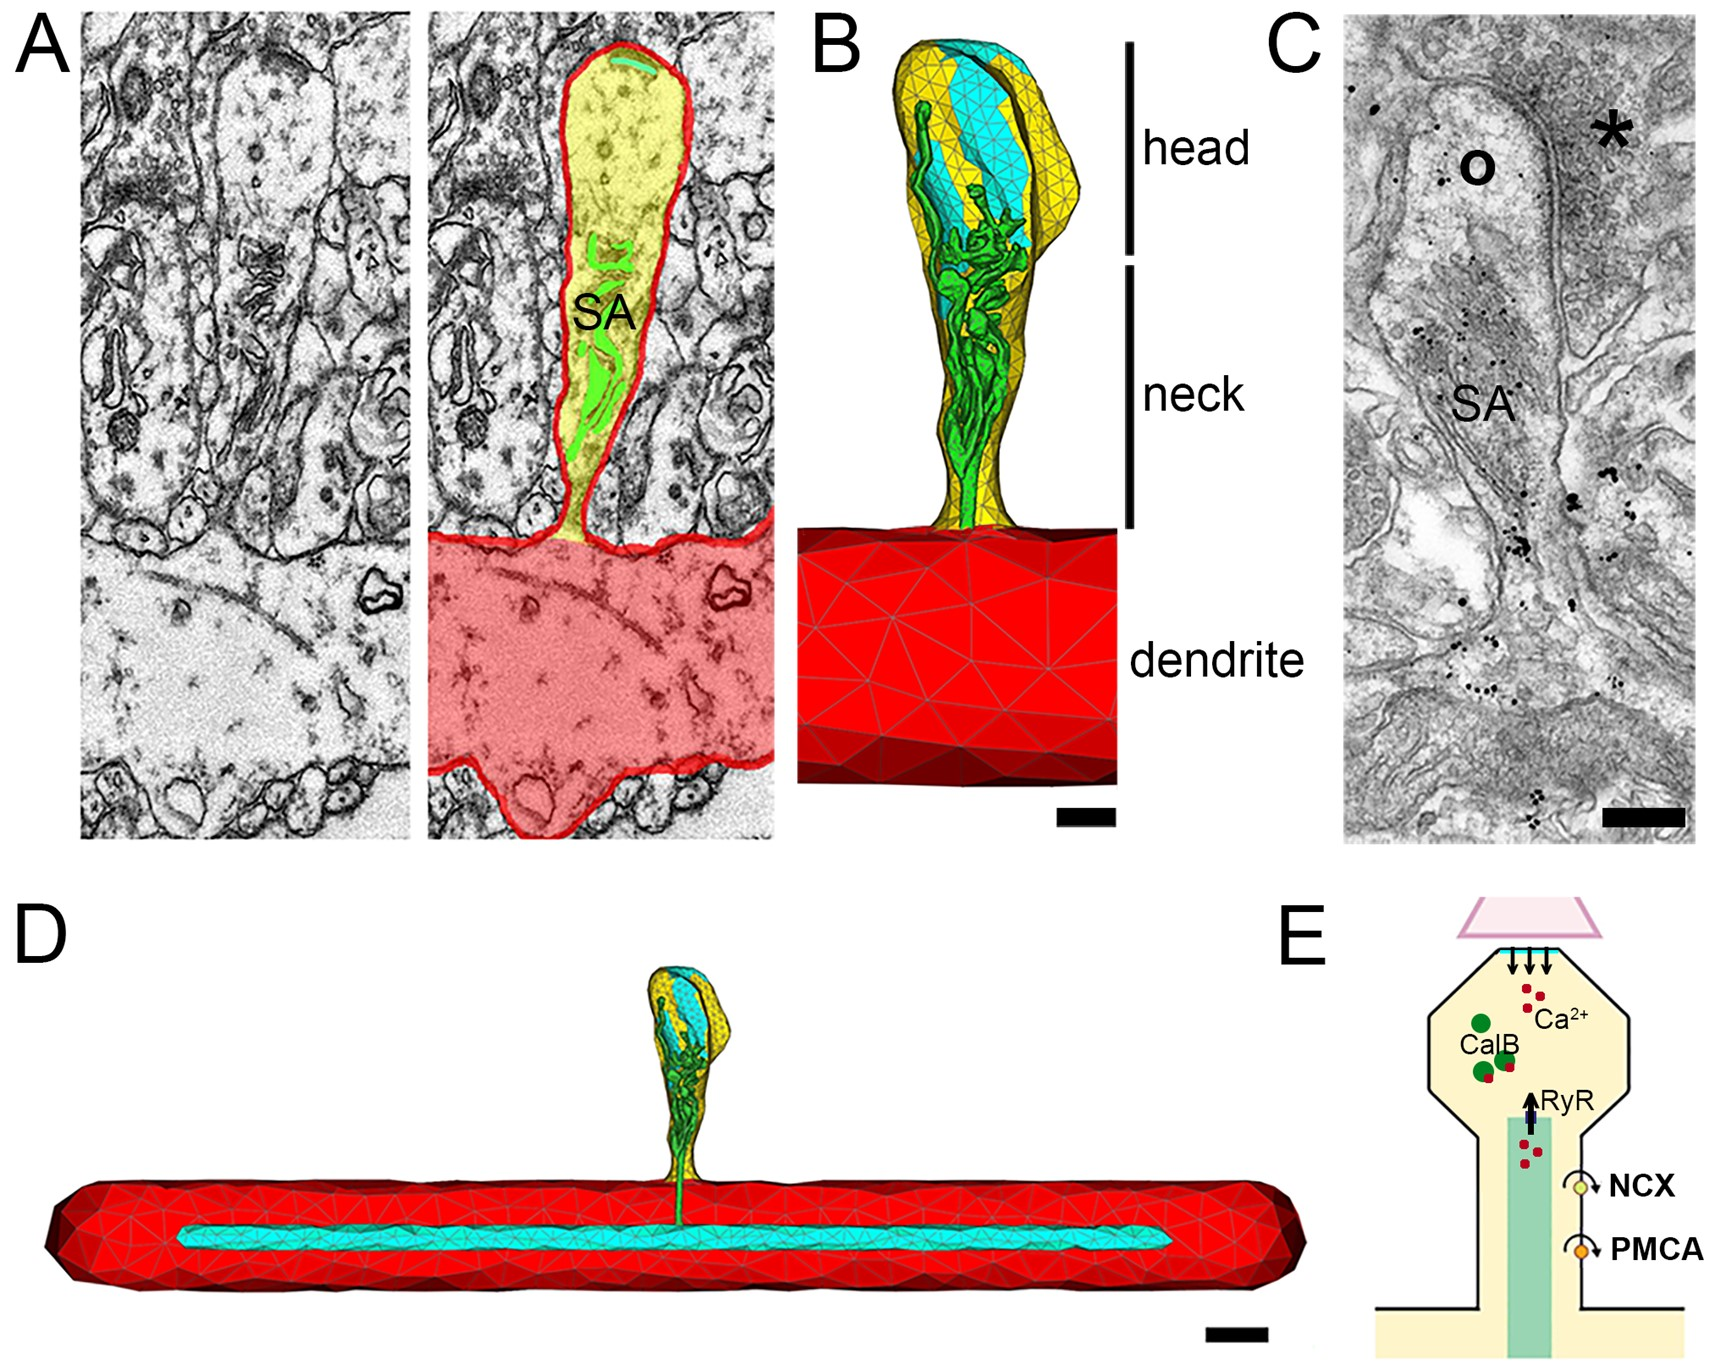
\includegraphics[width=0.85\linewidth]{figures/figure1.jpg}
    \caption{Dendritic spine reconstruction and $\textrm{Ca}^{2+}$ modeling. (A) Spine morphologies are based on serial reconstructions of transmission electron micrographs obtained from human cortical tissue. (B) An example of a reconstructed dendritic spine (dendrite, red; spine compartment, yellow) carrying a spine apparatus organelle (SA, green). Upon release of $\textrm{Ca}^{2+}$ at the reconstructed postsynaptic density (cyan), changes in $[\textrm{Ca}^{2+}]$ are determined in the head, neck and dendritic region, respectively. Scale bar, 200 nm. (C) Immunogold staining for the actin-binding protein synaptopodin \cite{Lenz2021}, which is a marker and essential component of the SA. Asterisk indicates presynaptic, circle the postsynaptic  compartment. Scale bar, 200 nm. (D) In all reconstructed human spines the SA was attached to a single standardized dendritic ER tubule in a dendritic compartment with identical dimensions. Scale bar, 500 nm. (E) The model accounts for $\textrm{Ca}^{2+}$ exchange mechanisms on the plasma membrane ($\textrm{Na}^{+}$/$\textrm{Ca}^{2+}$ exchangers (NCX), plasma membrane $\textrm{Ca}^{2+}$-ATPases (PMCA)) and on the ER (green; ryanodine-receptors (RyR)). Calcium buffering capacity (Calbindin, CalB) is kept constant. Further details on physiological values are provided in the main text and in Table \ref{table4}. Tables \ref{table1} and \ref{table3} contain morphological measurements such as surface area. See also supplemental movie.}
    \label{fig:fig1}
\end{figure}

\clearpage
\begin{figure}[ht]
    \centering
    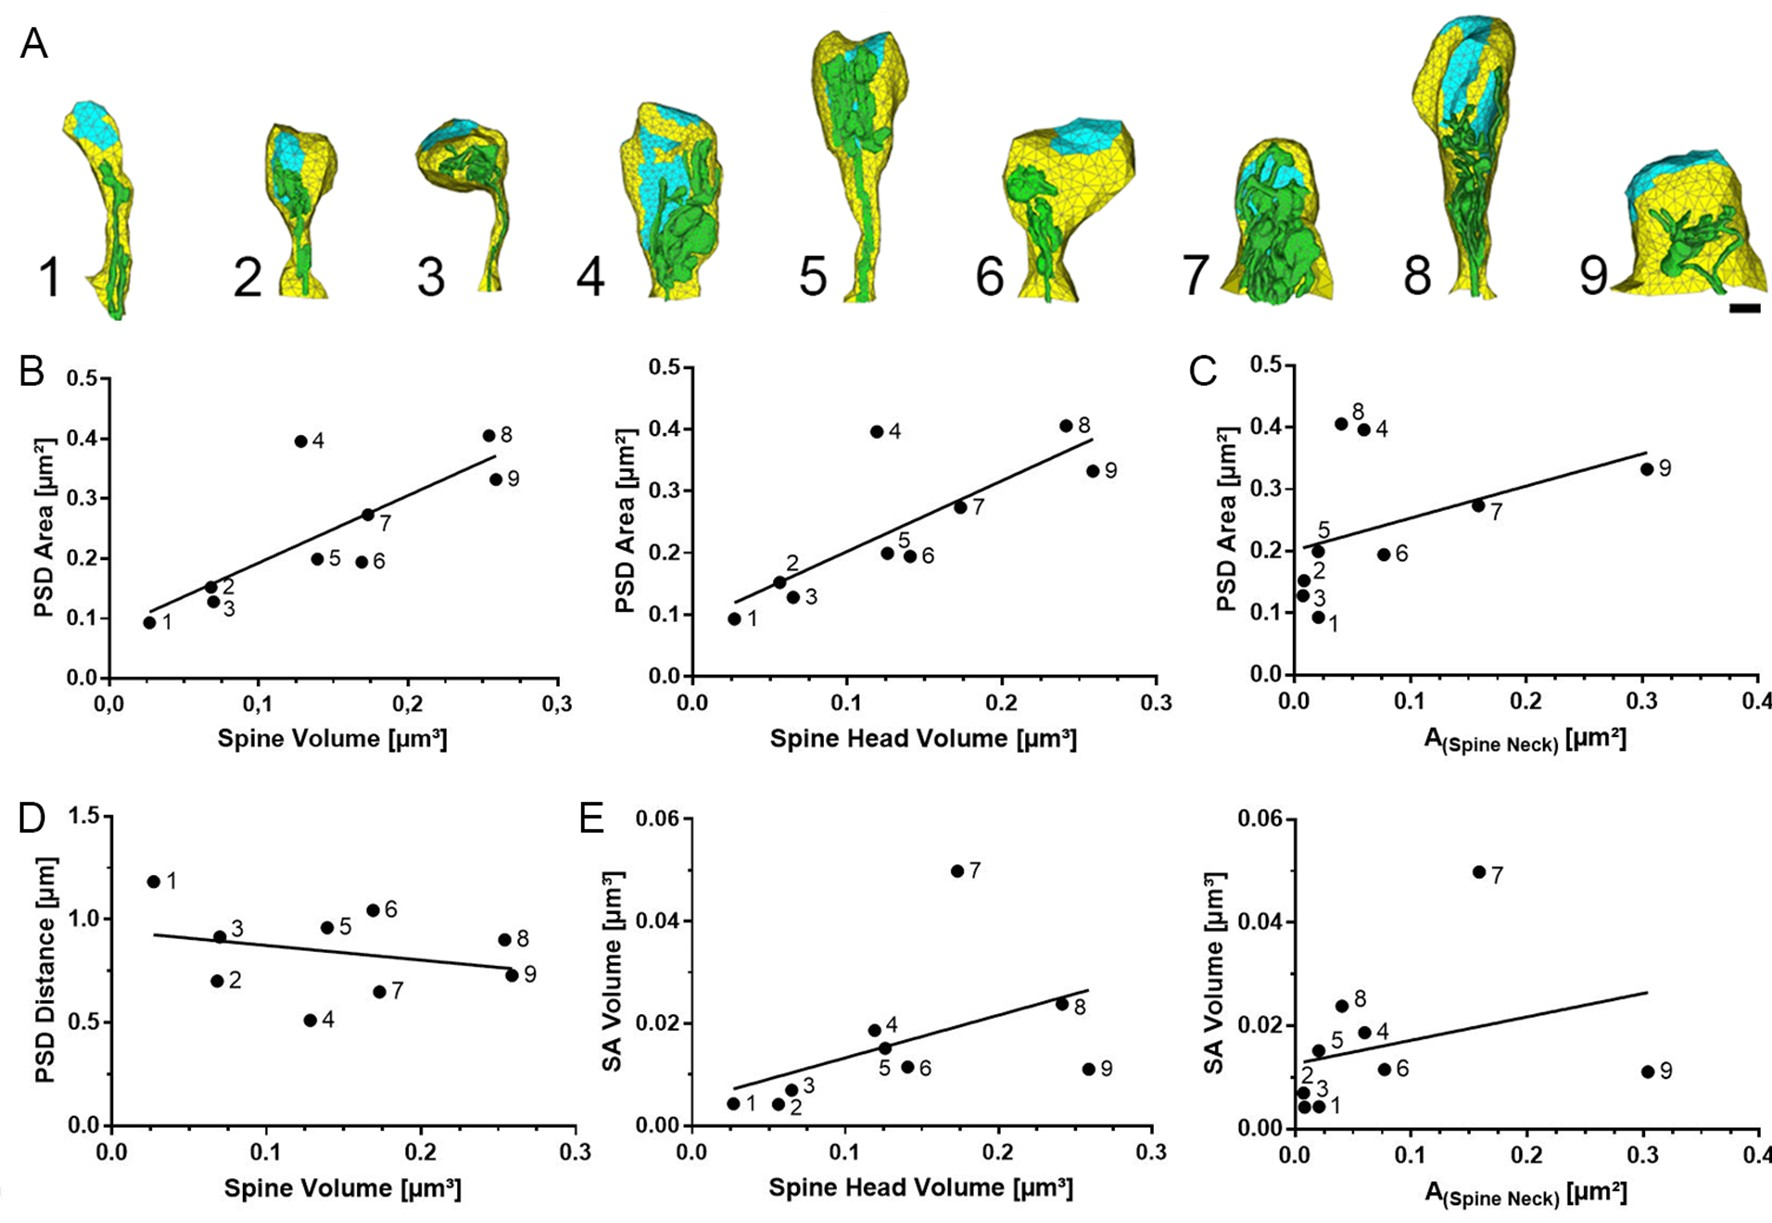
\includegraphics[width=\linewidth]{figures/figure2.jpg}
    \caption{Morphological parameter of reconstructed spines. (A) Three-dimensional models based on reconstructed human dendritic spines. Spine apparatus organelle, green. Postsynaptic density, cyan. Scale bar, 200 nm (B) Dendritic spines with large volumes have large postsynaptic densities. (C) Positive correlation between spine neck diameter and postsynaptic density sizes. (D) Postsynaptic densities in large spines are not further away from spine base. (E) Large spines contain large spine apparatus organelles, which are found in spines with wider spine necks. $n = 9$ reconstructed dendritic spines from 4 independent samples.}
    \label{fig:fig2}
\end{figure}

\clearpage
\begin{figure}[ht]
    \centering
    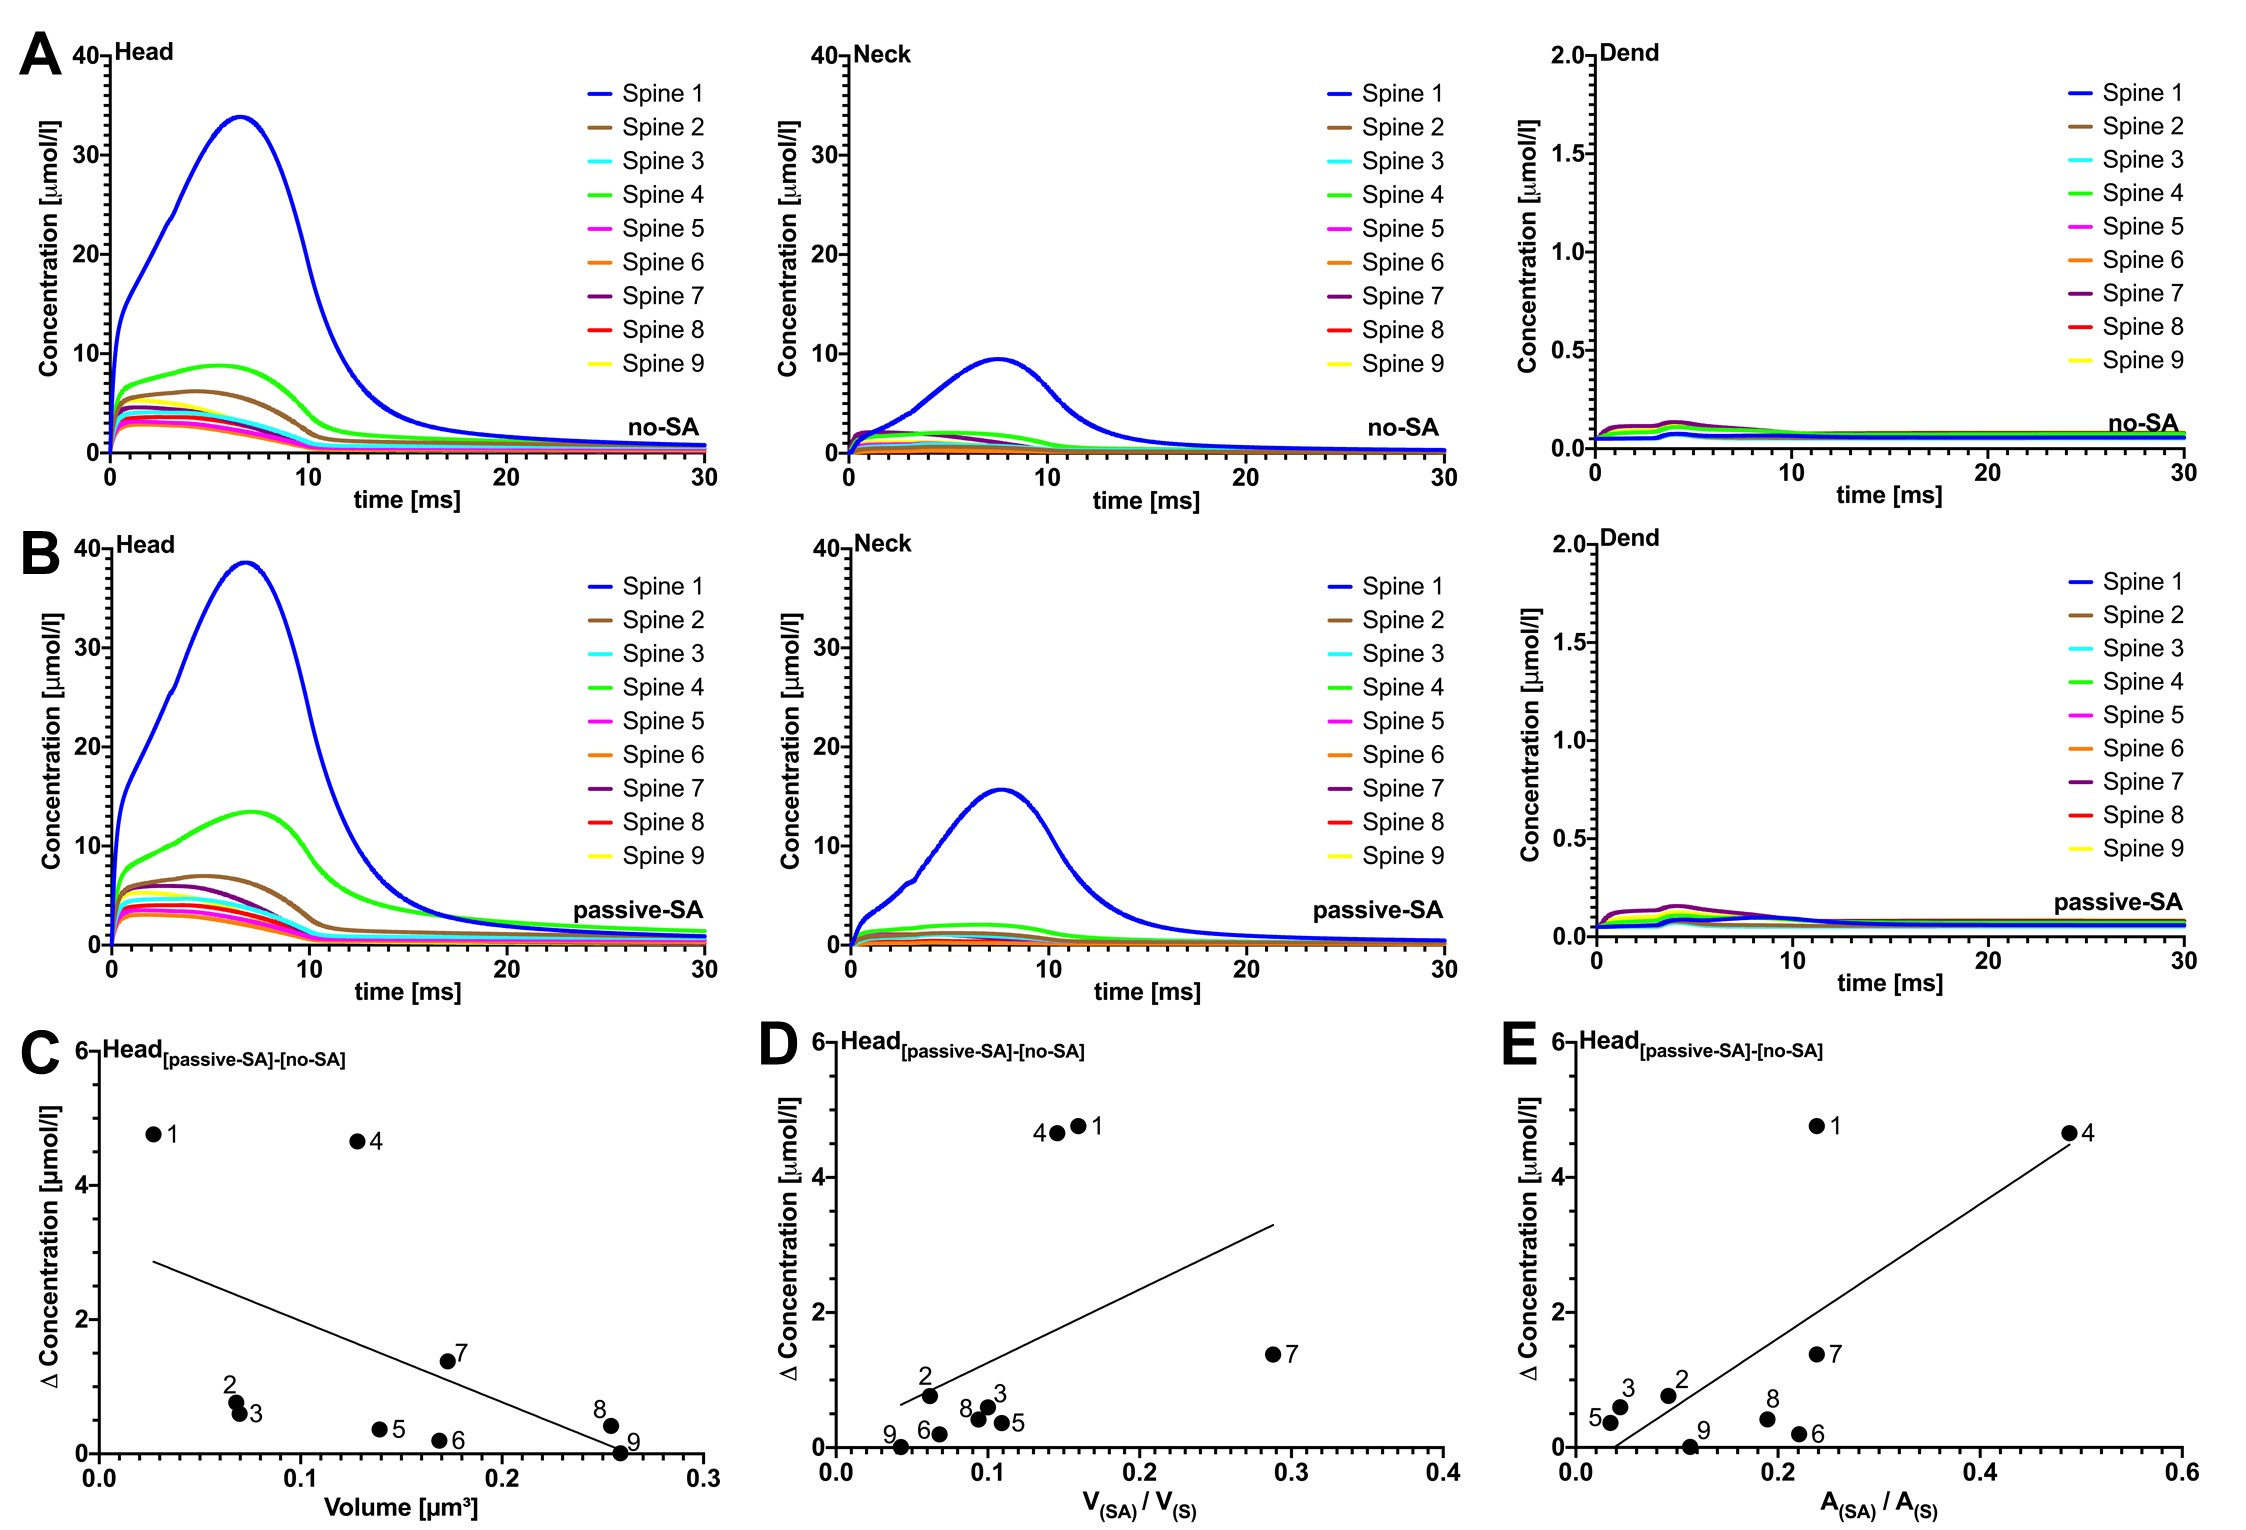
\includegraphics[width=\linewidth]{figures/figure3.jpg}
    \caption{Effects of passive spine SA on spine-to-dendrite $\textrm{Ca}^{2+}$ signaling, with fixed $\textrm{Ca}^{2+}$ influx.  Row A, without  SA, and row B, with SA, show $\textrm{Ca}^{2+}$ profiles for 10 ms initial $\textrm{Ca}^{2+}$ release into the spine head.  Consistent with experimental data, spine-to-dendrite $\textrm{Ca}^{2+}$ signaling does not occur for all 9 simulated spines, and this also holds true for simulations where $\textrm{Ca}^{2+}$ influx is adapted to the postsynaptic area, see additional plots. Row C (fixed $\textrm{Ca}^{2+}$ influx) demonstrates correlations between maximum $[\textrm{Ca}^{2+}]$ in the head region versus spine volume, ratio of SA area/Spine area, and SA volume/Spine volume. Presence of a passive SA, i.e., no Ryanodine receptors, has no major effect on $[\textrm{Ca}^{2+}]$ dynamics in the spine head and neck.}
    \label{fig:fig3}
\end{figure}

\clearpage
\begin{figure}[ht]
    \centering
    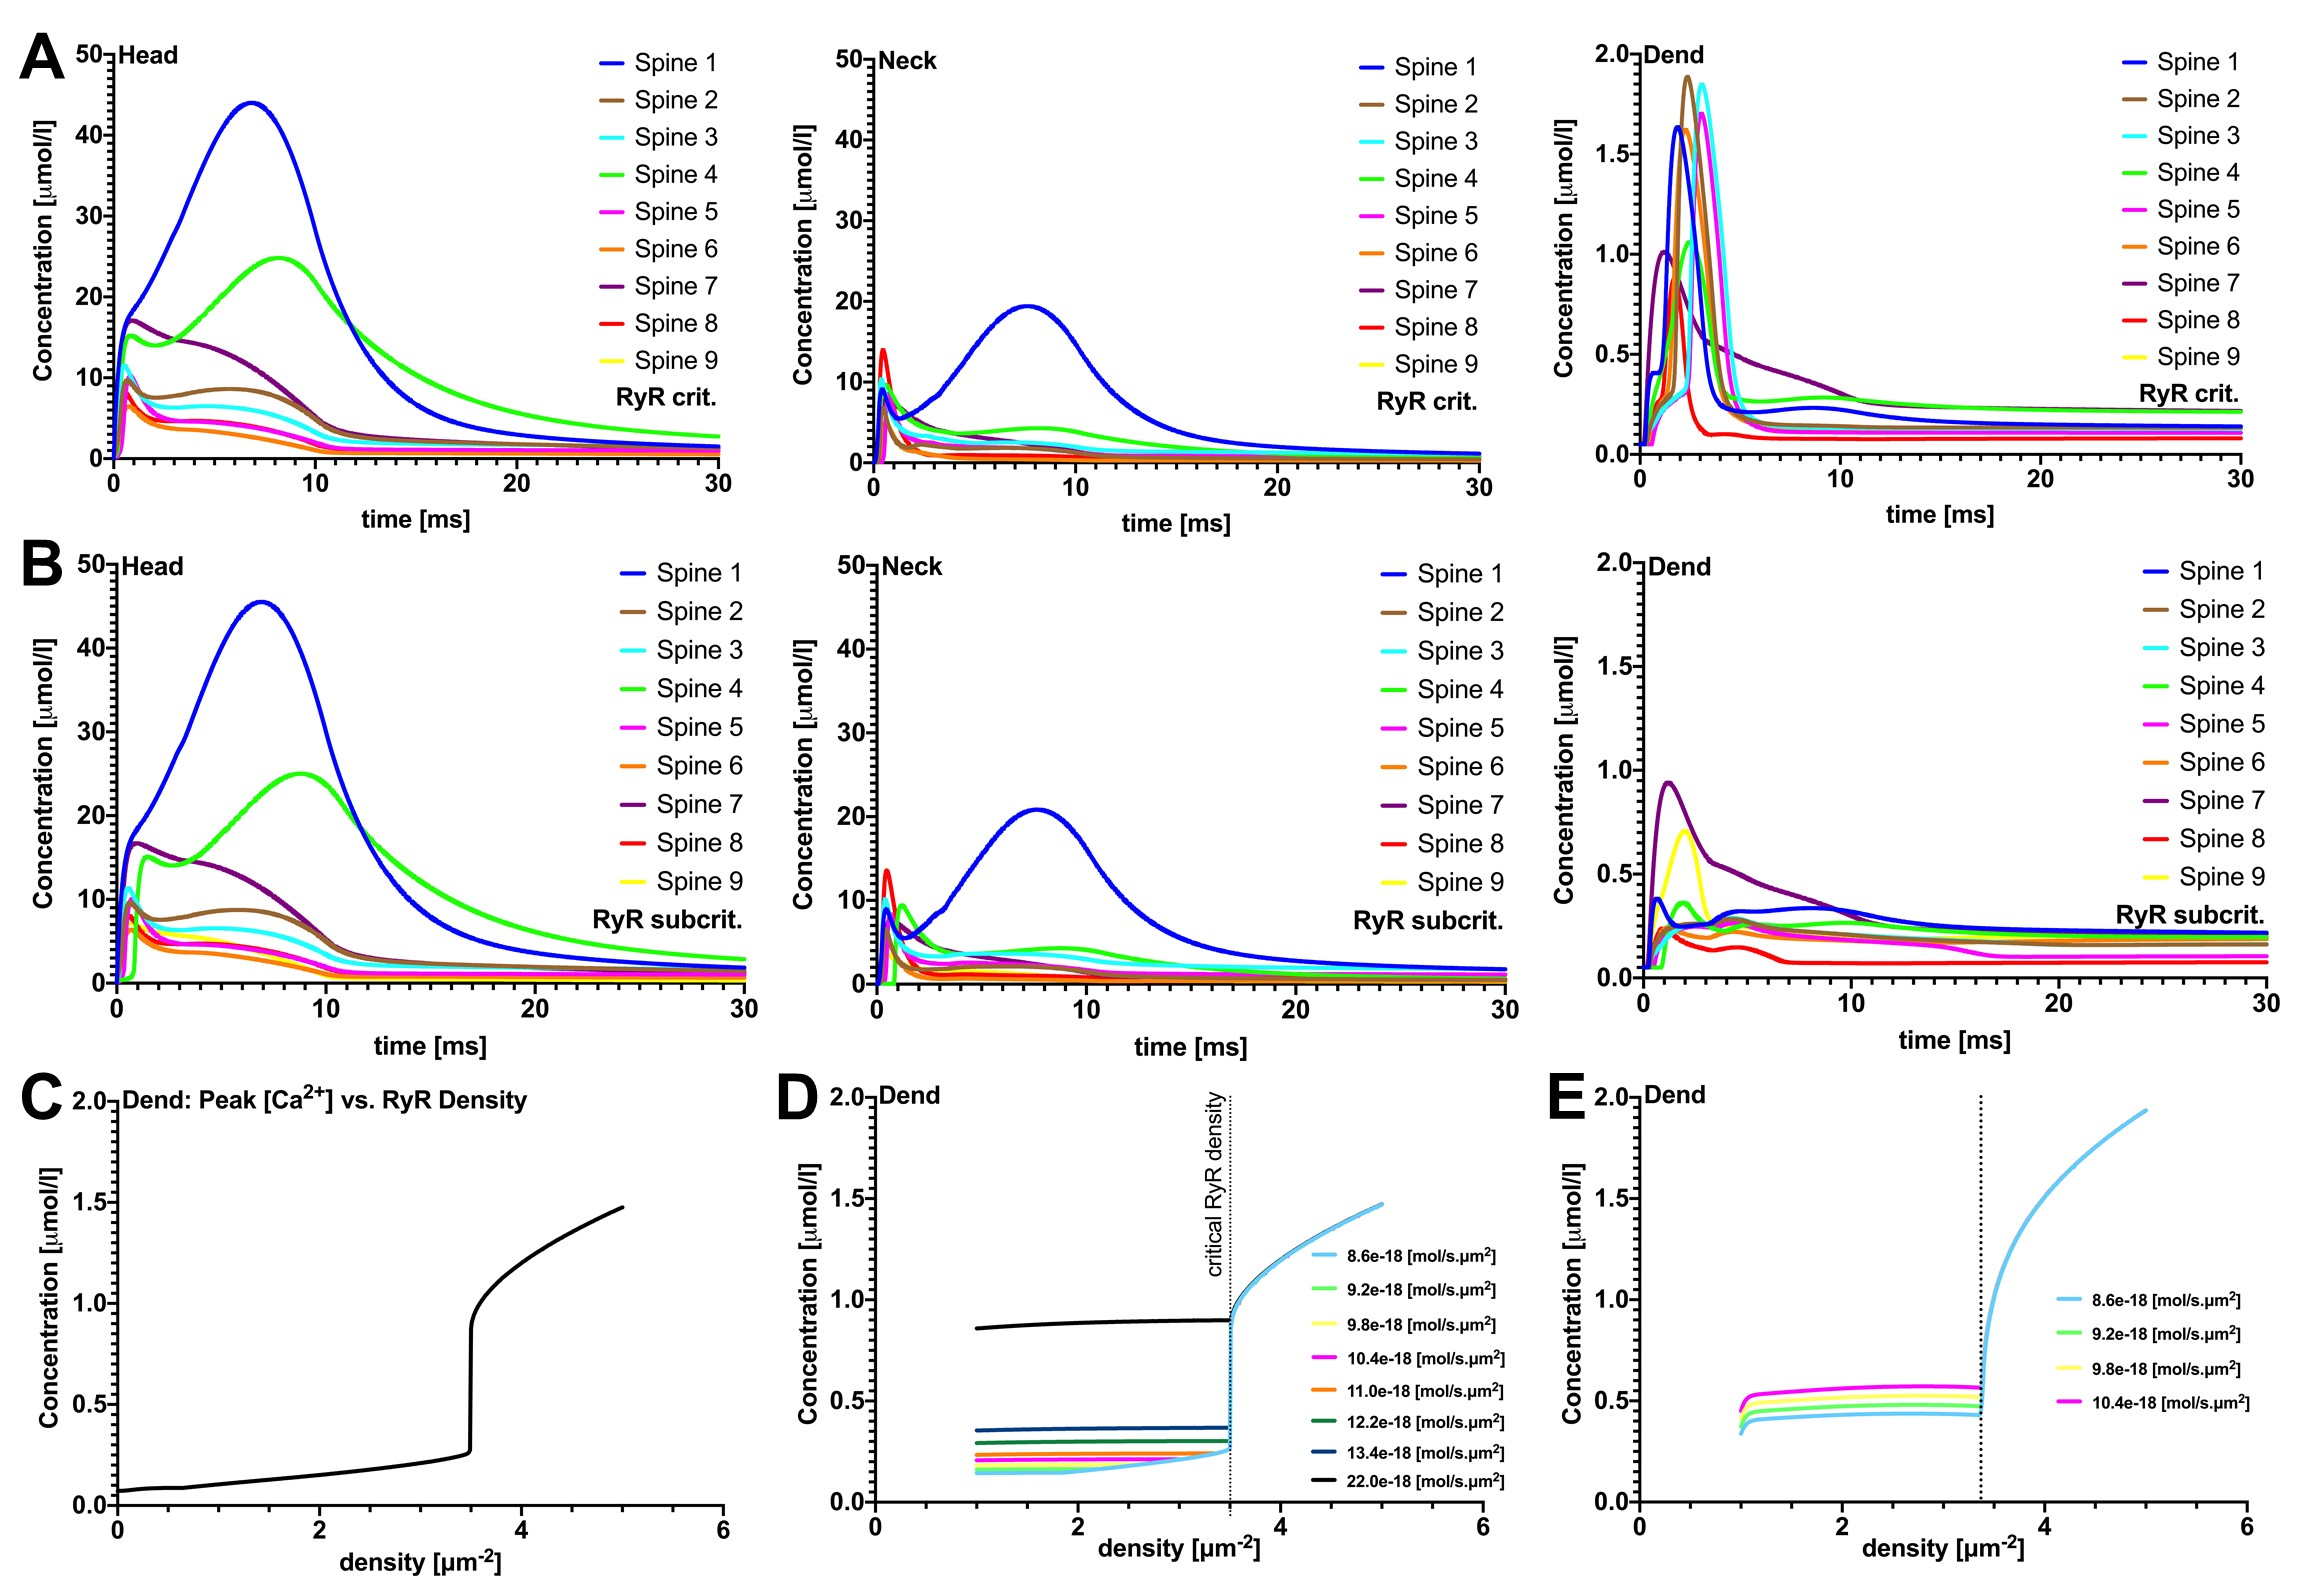
\includegraphics[width=\linewidth]{figures/figure4.jpg}
    \caption{Effects of active SA with RyR calcium exchange mechanisms only. These plots were generated with active SA with only ryanodine receptors. Plots in row A show the calcium concentration traces in the head and dendrite at the critical RyR density. Plots in row B show the calcium concentration traces at sub-critical (5\% below critical) RyR density. It is worth observing that $\textrm{Ca}^{2+}$ coupling is significantly decreased. In Figures 4C-4E, we demonstrate for spine 8 that there is a critical RyR density such that $\textrm{Ca}^{2+}$ coupling occurs in the dendritic region. The RyR density parameter is incremented in 0.01 $\mu m^{-2}$ increments. One can observe the maximum $[\textrm{Ca}^{2+}]$ in the dendritic region has a significant jump at $\approx$ 3.50 $\mu m^{-2}$. For plot D we performed the same RyR density increment experiments but with different $\textrm{Ca}^{2+}$ influx at the synapse. For all spine simulations (rows A and B) we used a fixed $\textrm{Ca}^{2+}$ influx at the synapse.}
    \label{fig:fig4}
\end{figure}

\clearpage
\begin{figure}[ht]
    \centering
    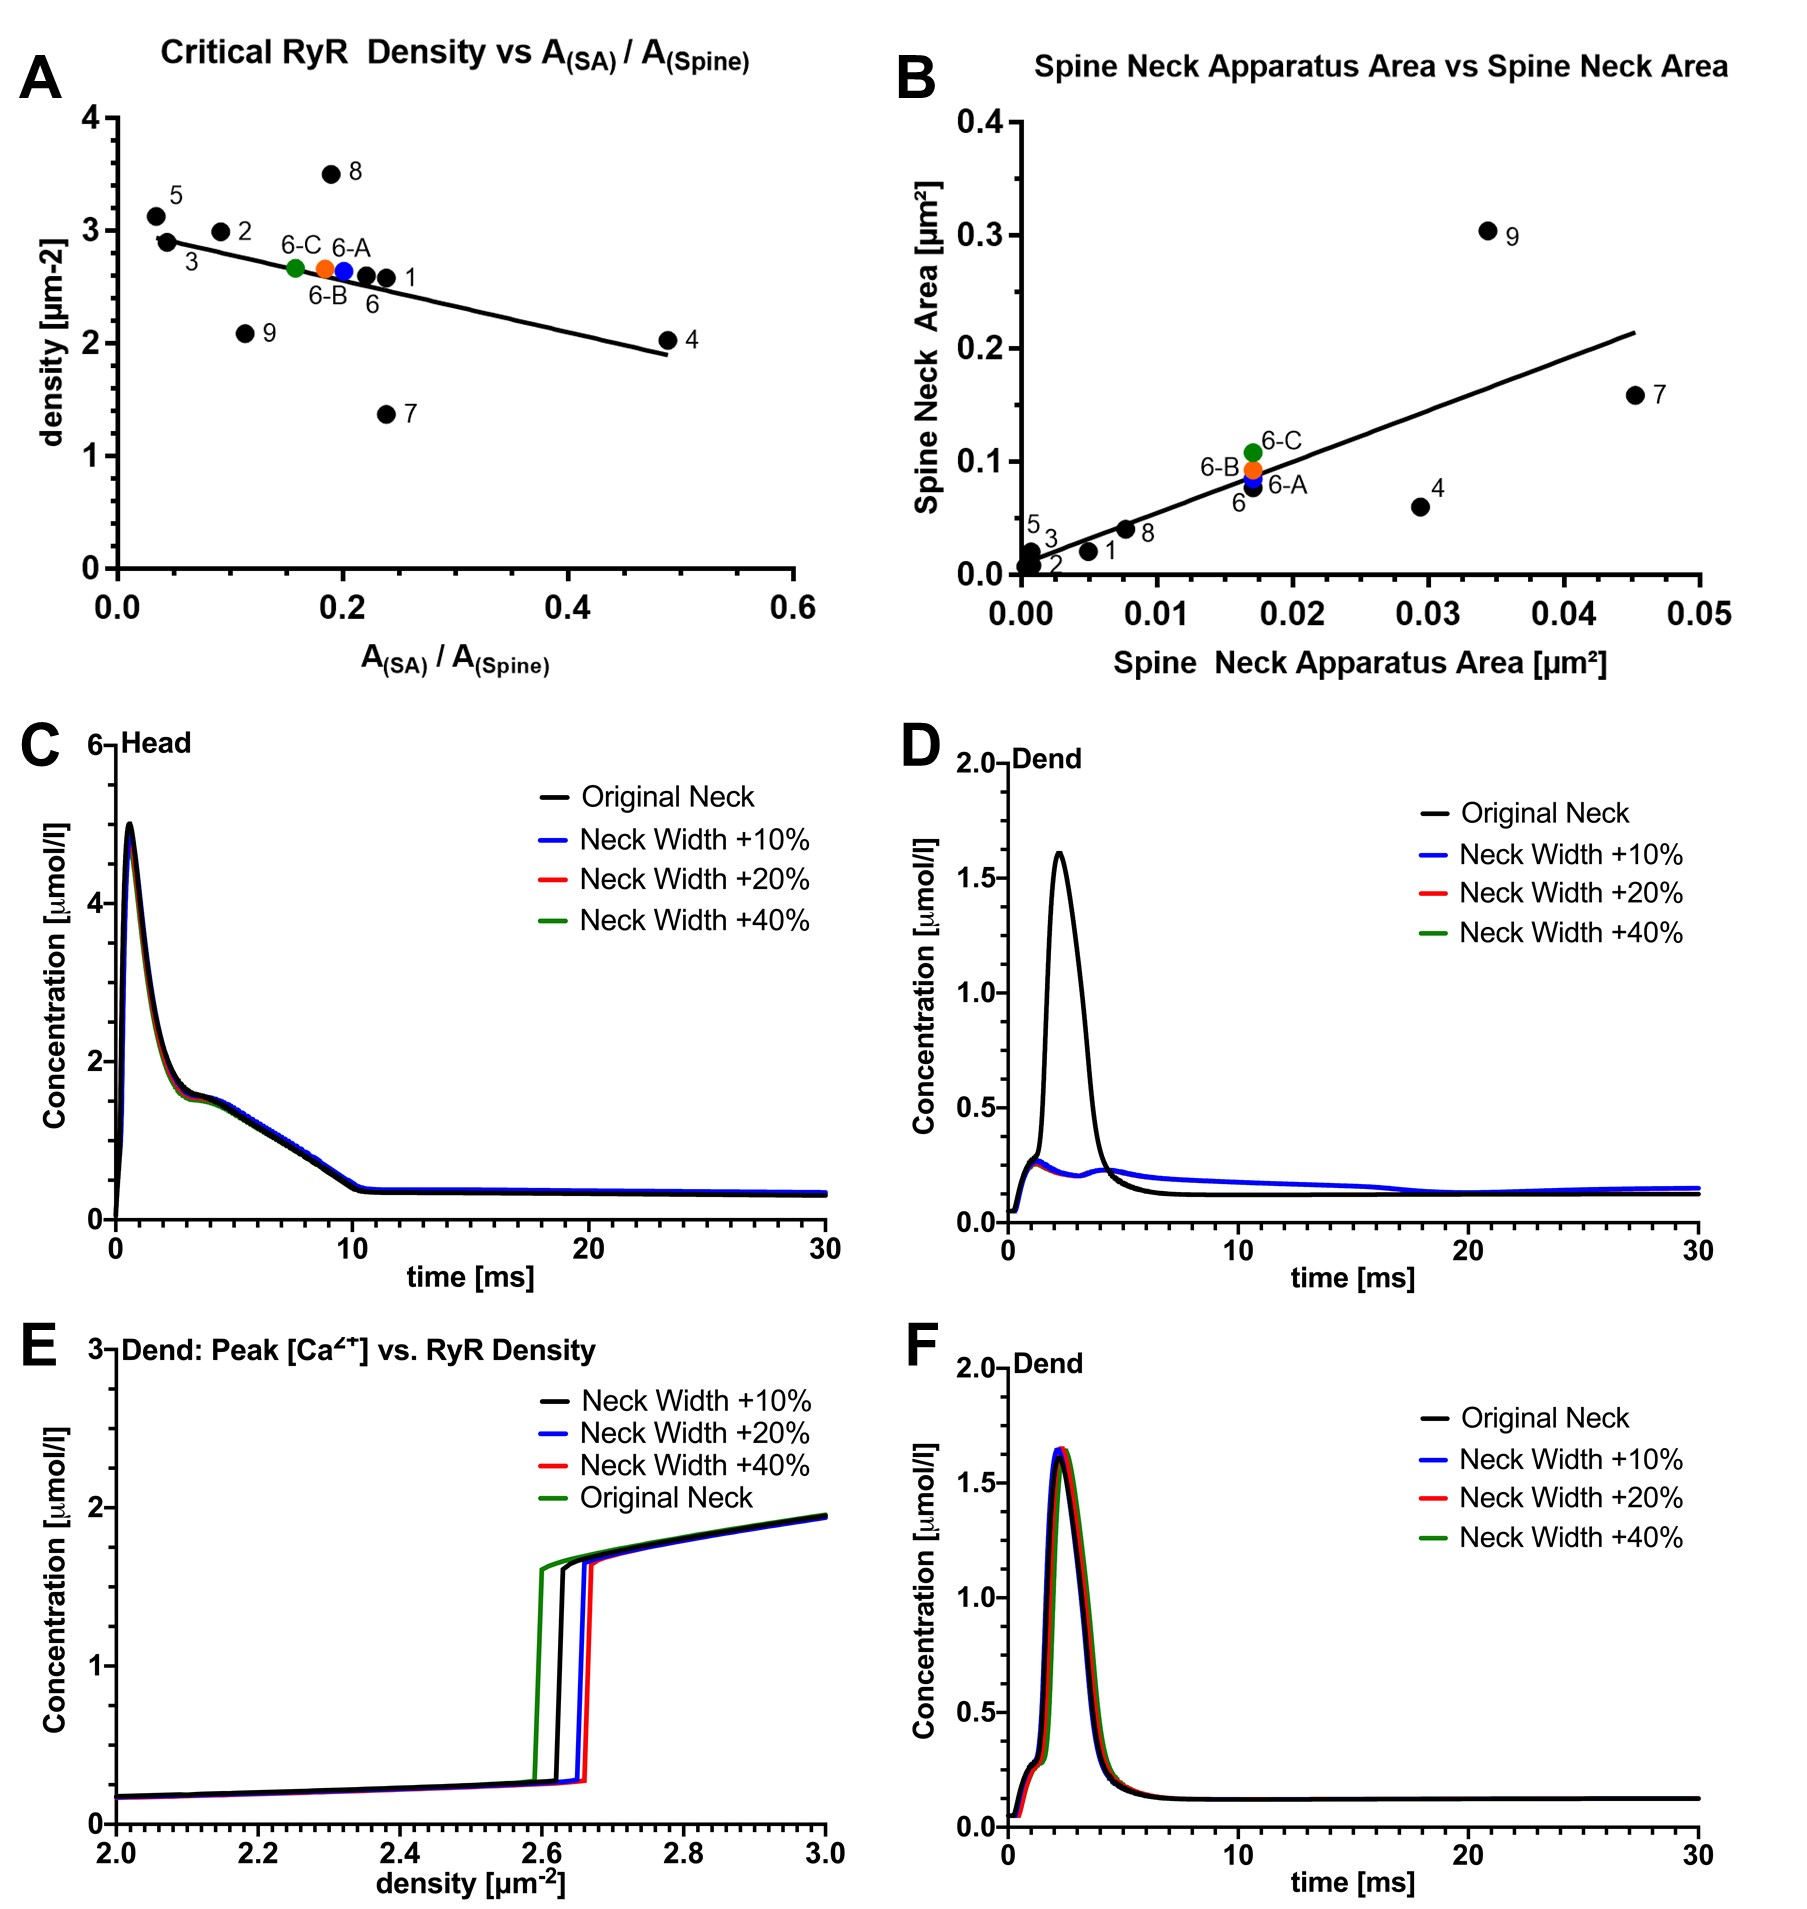
\includegraphics[width=0.75\linewidth]{figures/figure5.jpg}
    \caption{In A we plot the critical RyR density against the ratio of Spine Apparatus Neck area to Spine Neck area. In Table \ref{table1} we show the values that correspond to A. In C and D we demonstrate that widening the neck diameter of a spine affects the coupling of $\textrm{Ca}^{2+}$ to the dendritic region. In particular E indicates that neck widening causes the critical RyR density to increase.}
    \label{fig:fig5}
\end{figure}

\clearpage

\begin{figure}[ht]
    \centering
    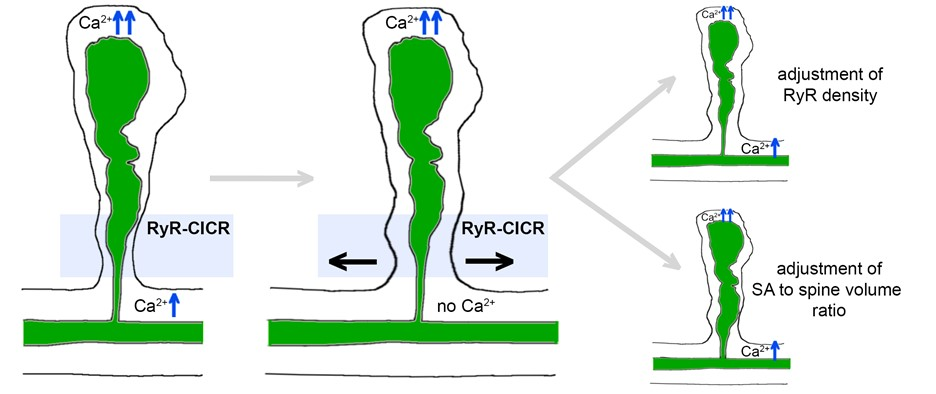
\includegraphics[width=\linewidth]{figures/figure8.jpg}
    \caption{
    ``All or-nothing'' spine-to-dendrite calcium communication. Schematic illustration summarizing our major findings. 
$\textrm{Ca}^{2+}$ communication between spine head and dendrite is controlled by the interplay between RyR density, and morphological changes of dendritic spines and spine apparatus organelles (SA) in the neck region. RyR, Ryanodine receptors.
    %Summary of morphological control of spine-to-dendrite $\textrm{Ca}^{2+}$ signaling. $\textrm{Ca}^{2+}$ diffusion is affected by changes in spine neck and SA geometry. Increasing the neck diameter or decreasing the SA cross-sectional area in the neck region of individual spines, while keeping the RyR density and the SA morphology constant, causes decoupling in spine-to-dendrite communication. In order to restore coupling spine neck plasticity can be counterbalanced by either increasing the RyR density or enlarging the SA size.
    }
    \label{fig:fig8}
\end{figure}

\begin{figure}[ht]
\renewcommand\thefigure{S1}
    \centering
    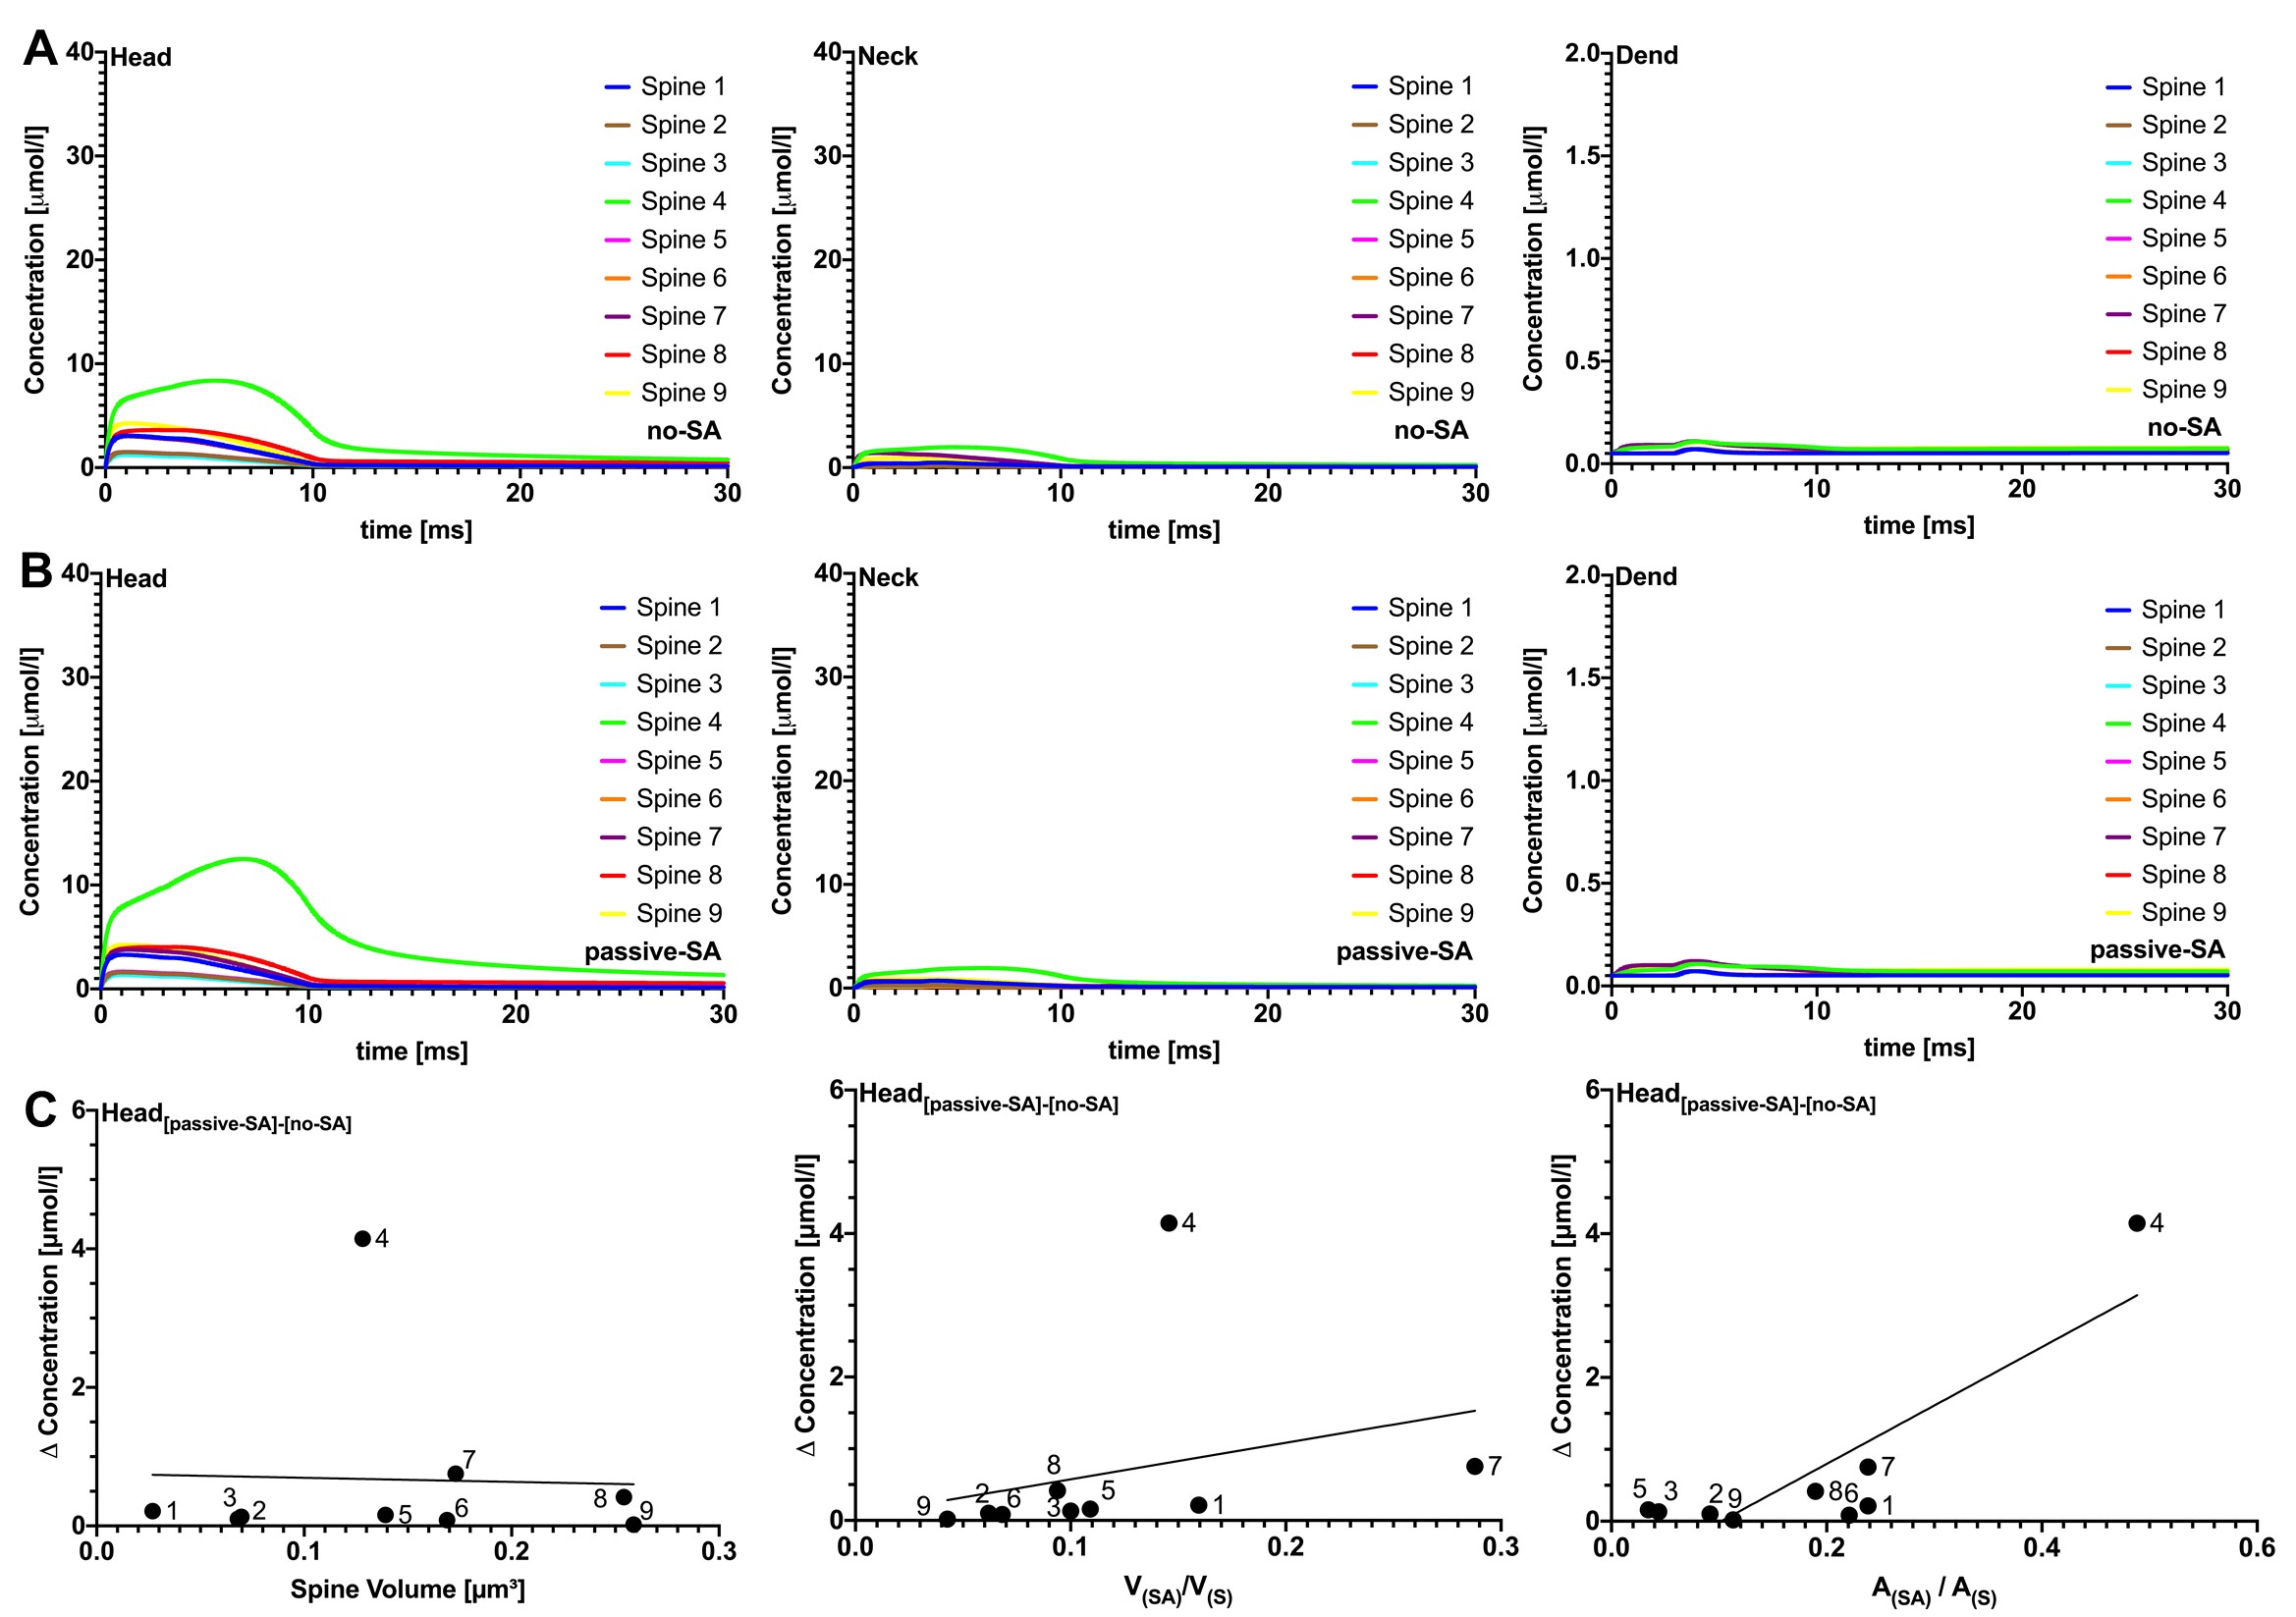
\includegraphics[width=\linewidth]{figures/figure7.jpg}
    \caption{Effects of passive spine SA on spine-to-dendrite $\textrm{Ca}^{2+}$ signaling, with PSD adjusted $\textrm{Ca}^{2+}$ influx.  Plots in row A are without SA and plots in row B are with SA, showing $\textrm{Ca}^{2+}$ profiles for 10 ms initial $\textrm{Ca}^{2+}$ release into the spine head.  Consistent with experimental data, spine-to-dendrite $\textrm{Ca}^{2+}$ signaling does not occur for all 9 simulated spines. Presence of a passive SA, i.e., no Ryanodine receptors, has no major effect on $\textrm{Ca}^{2+}$ dynamics in the spine head and neck.}
    \label{fig:fig7}
\end{figure}

\clearpage
\begin{figure}[ht]
\renewcommand\thefigure{S2}
    \centering
    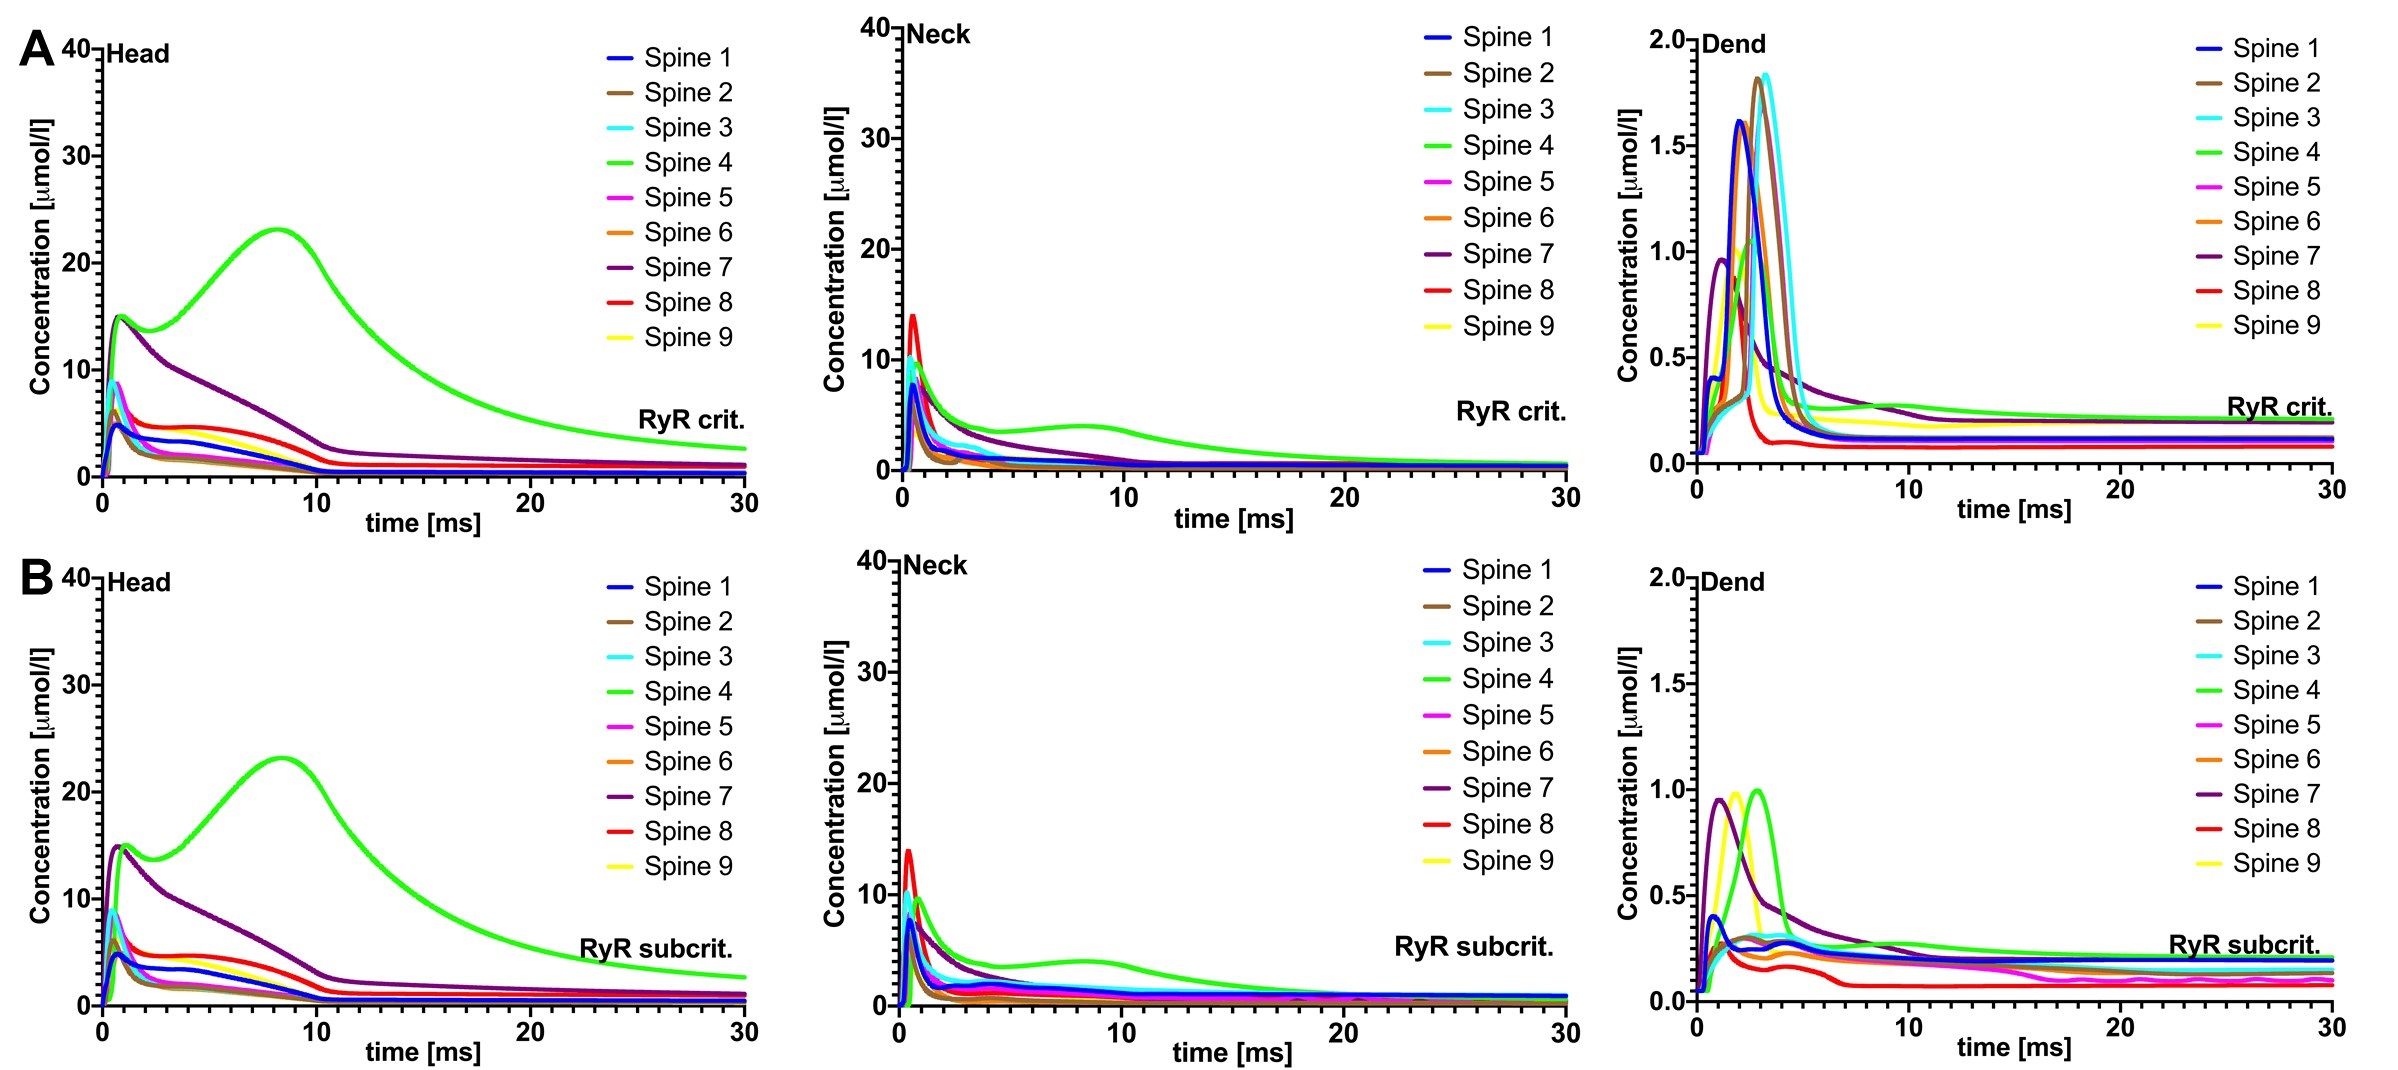
\includegraphics[width=\linewidth]{figures/figure6noserca.jpg}
    \caption{All plots were generated with PSD adjusted calcium influx. In row A, these are the calcium concentration profiles in the head and dendrite region %with SERCA pumps off and
    at critical RyR density. In row B, these calcium concentration profiles correspond to sub-critical RyR density. }
    %In row C, these are the calcium concentration profiles at critical RyR density with SERCA pumps on. In row C, when SERCA pumps are activated we observe oscillations in the some of the calcium concentration profiles}
    \label{fig:fig6}
\end{figure}
\clearpage

\begin{table}[h]
\resizebox{\textwidth}{!}{%
\begin{tabular}{|c|c|c|c|c|c|c|}
\hline
 & \multicolumn{3}{c|}{\textbf{Head}} & \multicolumn{3}{c|}{\textbf{Dendrite}} \\ \hline
\textbf{\begin{tabular}[c]{@{}c@{}}Spine \\ No.\end{tabular}} & \textbf{\begin{tabular}[c]{@{}c@{}}passive\\     peak $[\textrm{Ca}^{2+}]$\end{tabular}} & \textbf{\begin{tabular}[c]{@{}c@{}}active \\ peak $[\textrm{Ca}^{2+}]$\end{tabular}} & \textbf{\begin{tabular}[c]{@{}c@{}}\% \\  increase\end{tabular}} & \textbf{\begin{tabular}[c]{@{}c@{}}passive\\     peak $[\textrm{Ca}^{2+}]$\end{tabular}} & \textbf{\begin{tabular}[c]{@{}c@{}}active \\ peak $[\textrm{Ca}^{2+}]$\end{tabular}} & \textbf{\begin{tabular}[c]{@{}c@{}}\%  \\ increase\end{tabular}} \\ \hline
\textbf{1} & 33.85 & 44.00 & 30\% & 0.08 & 1.64 & 1,950\% \\ 
\textbf{2} & 6.22 & 9.66 & 55\% & 0.07 & 1.89 & 2,600\% \\ 
\textbf{3} & 4.09 & 11.47 & 180\% & 0.07 & 1.85 & 2,543\% \\ 
\textbf{4} & 8.80 & 24.82 & 180\% & 0.11 & 1.06 & 864\% \\ 
\textbf{5} & 3.16 & 10.22 & 223\% & 0.07 & 1.70 & 2,329\% \\ 
\textbf{6} & 2.86 & 6.47 & 126\% & 0.07 & 1.62 & 2,214\% \\ 
\textbf{7} & 4.60 & 17.09 & 270\% & 0.14 & 1.01 & 621\% \\ 
\textbf{8} & 3.62 & 8.11 & 124\% & 0.07 & 0.88 & 115\% \\
\textbf{9} & 5.29 & 7.20 & 36\% & 0.12 & 1.05 & 775\% \\ \hline
\end{tabular}%
}
\caption{All concentrations are measured in $\mu \textrm{mol}/l$.}
\label{table2}
\end{table}
\clearpage

% Please add the following required packages to your document preamble:
% \usepackage{graphicx}
\begin{table}[ht]
\resizebox{\textwidth}{!}{%
\begin{tabular}{|c|c|c|c|c|c|c|}
\hline \textbf{\begin{tabular}[c]{@{}c@{}}Spine \\ No.\end{tabular}} & \textbf{\begin{tabular}[c]{@{}c@{}}RyR Critical   \\ Density $\mu m^{-2}$\end{tabular}} & \textbf{\begin{tabular}[c]{@{}c@{}}SA Surface   \\ Area \end{tabular}} & \textbf{\begin{tabular}[c]{@{}c@{}}SA + Tube   \\ Surface Area\end{tabular}} & \textbf{\begin{tabular}[c]{@{}c@{}}No. RyRs\\    (SA only)\end{tabular}} & \textbf{\begin{tabular}[c]{@{}c@{}}No. RyRs\\    (SA + Tube)\end{tabular}} \\ \hline
\textbf{1}  & 2.58 & 0.3775 & 5.2696 & 1 & 14 \\
\textbf{2}  & 2.99 & 0.3607 & 5.6055 & 1 & 17 \\
\textbf{3}  & 2.90 & 0.5867 & 5.8341 & 2 & 17 \\
\textbf{4}  & 2.03 & 1.1270 & 6.3761 & 2 & 13 \\
\textbf{5} & 3.13 & 1.0291 & 6.2729 & 3 & 20 \\
\textbf{6}  & 2.60 & 0.6807 & 5.9312 & 2 & 15 \\
\textbf{6A} & 2.64 & 0.7092 & 5.9596 & 2 & 16 \\
\textbf{6B} & 2.66 & 0.7220 & 5.9724 & 2 & 16 \\
\textbf{6C} & 2.67 & 0.7347 & 5.9852 & 2 & 16 \\
\textbf{7} & 1.37 & 2.3209 & 7.5629 & 3 & 10 \\
\textbf{8} & 3.50 & 1.7146 & 6.6048 & 6 & 23 \\
\textbf{9} & 2.09 & 0.9134 & 5.8054 & 2 & 12 \\
\hline
\end{tabular}%
}
\caption{Surface area is in units of $\mu m^2$.} 
%The second column shows the number Ca$^{2+}$ ions released through the PSD during 10 ms release.}
\label{table1}
\end{table}

\clearpage

% Please add the following required packages to your document preamble:
% \usepackage{graphicx}
\begin{table}[ht]
\centering
{%
\begin{tabular}{|c|c|c|c|}
\hline
\textbf{\begin{tabular}[c]{@{}c@{}}Spine   \\ No.\end{tabular}} & \textbf{\begin{tabular}[c]{@{}c@{}}Area\\ SA Neck\end{tabular}} & \textbf{\begin{tabular}[c]{@{}c@{}}Area\\ Spine Neck\end{tabular}} & \textbf{\begin{tabular}[c]{@{}c@{}}Cross Section\\ Ratio {[}\%{]}\end{tabular}} \\ \hline
\textbf{3} & 0.0003265 & 0.0074247 & 4.4 \\ 
\textbf{5} & 0.0007031 & 0.0205083 & 3.4 \\ 
\textbf{2} & 0.0007682 & 0.0083852 & 9.2 \\ 
\textbf{1} & 0.0049353 & 0.0206937 & 23.8 \\ 
\textbf{8} & 0.0076741 & 0.0404725 & 19.0 \\ 
\textbf{6} & 0.0170800 & 0.0772860 & 22.1 \\ 
\textbf{4} & 0.0294116 & 0.0602114 & 48.8 \\ 
\textbf{9} & 0.0343718 & 0.3041610 & 11.3 \\ 
\textbf{7} & 0.0452300 & 0.1587200 & 28.5 \\ \hline
\end{tabular}%
}
\caption{Surface area is in units of $\mu m^2$.}
\label{table3}
\end{table}
\clearpage

\begin{table}[ht]
\centering
\resizebox{0.75\textwidth}{!}{%
\begin{tabular}{|ll||ll|}
\hline
\multicolumn{2}{|l||}{\textbf{Initial and equilibrium values}} & \multicolumn{2}{l|}{\textbf{PMCA pumps}} \\ \hline
$c_c$ & 50 nM & $I_p$ & $1.7\times 10^{-23}$ $\textrm{mol} \cdot s^{-1}$ \\
$c_e$ & 250 $\mu$M & $K_p$ & 60 nM \\
$c_o$ & 2 mM & $\rho_p$ & 500 $\mu m^{-2}$ \\ \cline{3-4} 
$p$ & 40 nM & \multicolumn{2}{l|}{\textbf{NCX pumps}} \\ \cline{3-4} 
$b^{tot}$ & 40 $\mu$M & $I_N$ & $2.5\times 10^{-21}$ $\textrm{mol}\cdot s^{-1}$ \\ \cline{1-2}
\multicolumn{2}{|l||}{\textbf{Diffusion/reaction}} & $K_N$ & 1.8 $\mu$ M \\ \cline{1-2}
$D_c$ & 220 $\mu m^2\cdot s^{-1}$ & $\rho_N$ & $15 \ \mu m^{-2}$ \\ \cline{3-4} 
$D_p$ & $280\ \mu m^2\cdot s^{-1}$ & \multicolumn{2}{l|}{\textbf{Leakage}} \\ \cline{3-4} 
$D_b$ & $20\ \mu m^2\cdot s^{-1}$ & $v_{l,e}$ & $38\ nm \cdot s^{-1}$ \\
$\kappa_b^-$ & $19\ s^{-1}$ & $v_{l,p}$ & $4.5\ nm \cdot s^{-1}$ \\
$\kappa_b^+$ & $27\ \mu \textrm{M}^{-1}s^{-1}$ &  &  \\ \cline{3-4} 
$\kappa_p$ & $0.11\ s^{-1}$ & \multicolumn{2}{l|}{\textbf{Calcium release}} \\ \cline{3-4} 
$p^r$ & 40 nM & $j_c^{rls}$ & $8.6\times 10^{-18}\ \textrm{mol}\cdot s^{-1} \mu m^{-2}$ \\ \cline{1-2}
\multicolumn{2}{|l||}{\textbf{RyR channel}} & $\tau_{rls}$ & $10\ ms$ \\ \cline{1-4}  %\hline
$k_a^-$ & $28.8\ s^{-1}$ & & \\ 
$k_a^+$ & $1500\ \mu \textrm{M}^{-4}\cdot s^{-1}$ & & \\ %$j_c^{rls}$ & $8.6\times 10^{-18}\ \textrm{mol}\cdot s^{-1} \mu m^{-2}$ \\
$k_b^-$ & $385.9\ s^{-1}$ & & \\ %$\tau_{rls}$ & $10\ ms$ \\
$k_b^+$& $1500 \mu\textrm{M}^{-3}\cdot s^{-1}$ & & \\ %$\tau_{NMDAR}$ & $150\ ms$ \\
$k_c^-$& $0.1\ s^{-1}$ & & \\ %$p_{NMDAR}$ & $8.15\times 10^{-3}\ \mu m^3\cdot s^{-1}$ \\
$k_c^+$ & $1.75\ s^{-1}$ &  &  \\
$\rho_r$ & $0.0 - 5.0\ \mu m^{-2}$ &  &  \\
$I_R^{ref}$ & $3.5\times 10^{-18}\ \textrm{mol}\cdot s^{-1}$ &  &  \\ \hline
\end{tabular}%
}
\caption{Constants used in simulations are borrowed from \cite{Breit2018}.}
\label{table4}
\end{table}

\clearpage
 \bibliography{export}
 \bibliographystyle{unsrt} 
\end{document}
